% !TeX root = ../main.tex

\chapter{概要设计}
本章在第3章需求分析的基础上,对运行时优化系统的设计进行初步介绍。首先将大的需求解耦,划分成不同的模块,然后对模块的内部功能和对外接口进行设计,相互配合依赖,达到系统最终的目的。

\section {总体设计}
\subsection {主流程优化}
分析DNNCL的运行流程,我们可以将其总结概括为以下几个步骤:构建计算图,动态编译,拷入数据,执行计算,拷出结果。结合需求分析,决定将优化措施分布在这几个步骤之中。如图~\ref{fig:main-process}所示,蓝颜色的是原流程的内容,黄色的表示优化的内容。

\begin{figure}[htb]
  \centering
  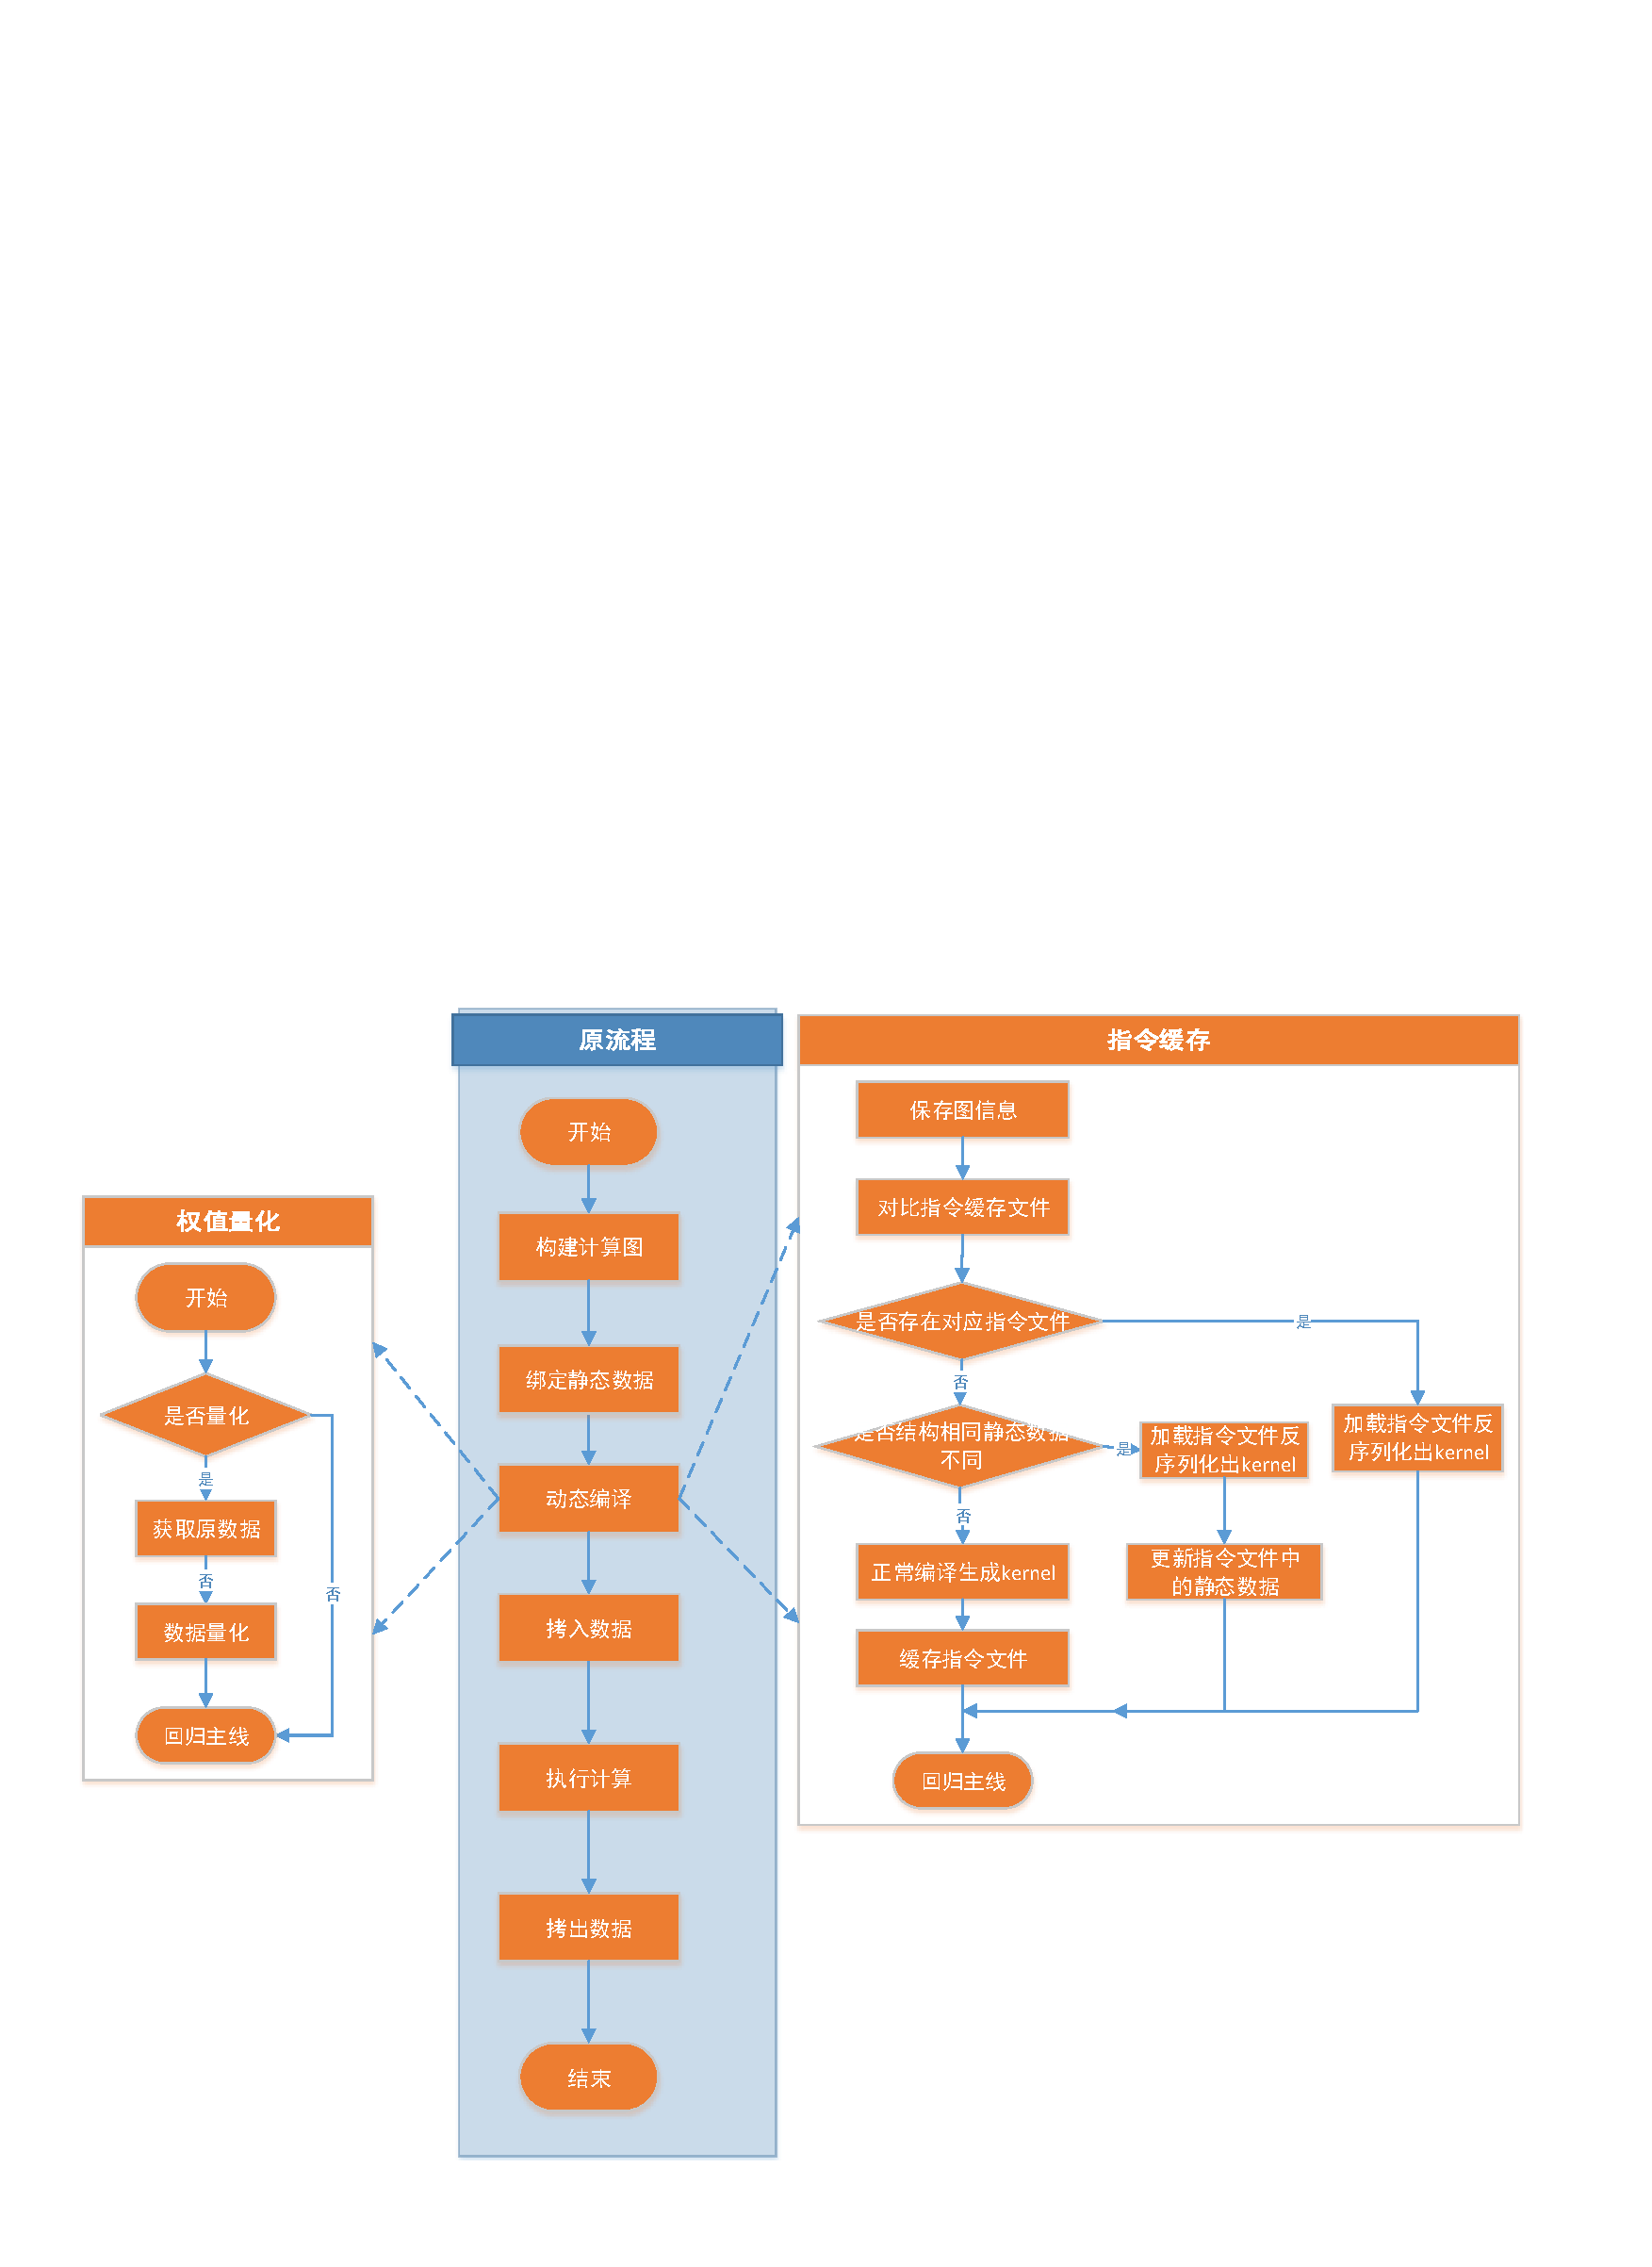
\includegraphics[width=0.8\textwidth]{main_process.pdf}
  \caption{运行时流程优化前后对比图}
  \label{fig:main-process}
\end{figure}

在动态编译过程中,引入权值量化。如果用户为了性能允许对权值等静态数据进行量化,则获取到原始用户传进来的数据,对原始数据进行精度量化,然后保存量化后的数据,节省网络的存储空间。

如果用户允许使用指令缓存功能,则在动态编译阶段,引入编译优化流程。在编译优化过程中,首先保存环境信息,环境信息包括硬件环境和软件环境,软件环境简可以直接用库版本信息表示。如果前后两次环境信息不一致,必须重新编译。其次是保存计算图信息,计算图信息也由两部分组成,第一个是用户传进来的神经网络的结构信息,保存神经网络的拓扑结构,第二部分是用户绑定的静态数据,静态数据包含权值和偏置值。如果结构信息和静态数据全和之前的一致,则可以直接加载以前缓存的指令,如果仅仅是静态数据变了,在更新静态数据后加载指令即可,如果结构信息和数据信息都不一致,则需要重新编译,并缓存这次编译好的指令作为备用。

\subsection {模块分解}
整个运行时优化可以分为三部分,编译优化,I/O优化和内存优化。针对每一个部分,都能做一定的优化措施,以便提升整体的运行流程。本系统主要从编译优化和内存优化的角度考虑。编译优化模块的主要目标是避免相同神经网络的重复编译,减少编译时间,节约编译资源;内存优化的主要目标是提升内存的利用率。为了实现编译优化和内存优化的目的,将主目标拆解,分为图信息识别模块、图信息保存模块、指令保存和加载模块、权值替换模块、指令替换模块、权值量化模块,模块分解如图~\ref{fig:model-split}所示。

\begin{figure}[htb]
  \centering
  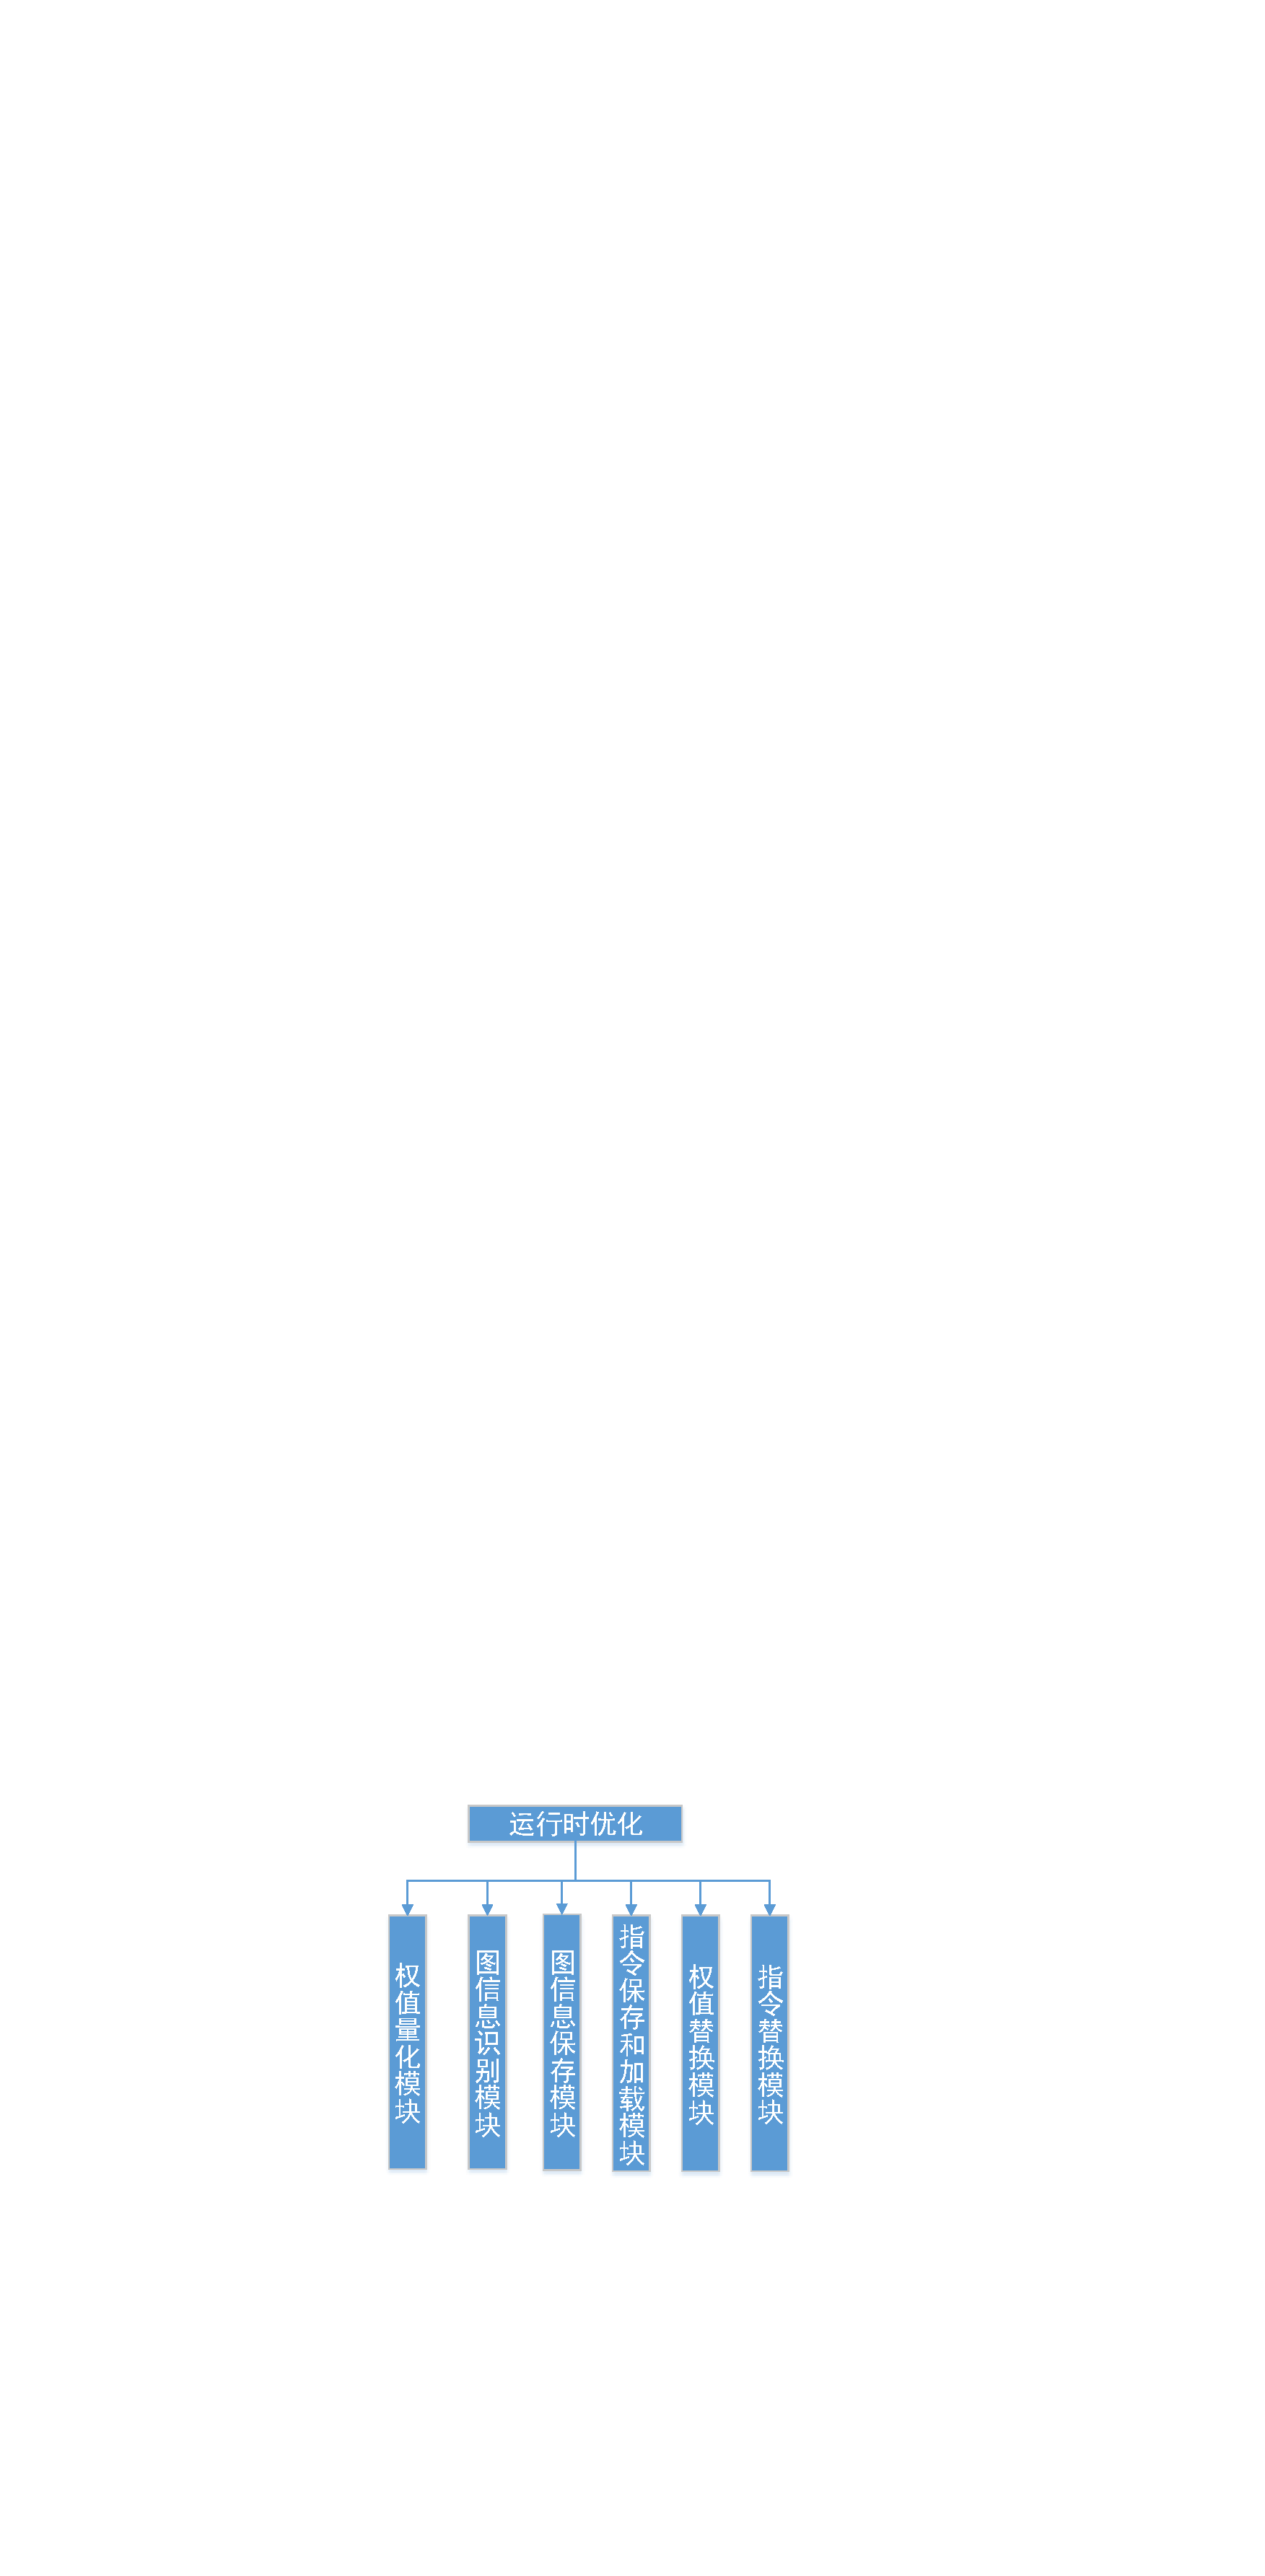
\includegraphics[width=0.6\textwidth]{model_split.pdf}
  \caption{模块分解图}
  \label{fig:model-split}
\end{figure}

\section {图信息保存模块}
\subsection {功能概述}
计算图信息保存模块是整个动态编译优化的基础,DNNCL库是声明式编程模式,用户所有的计算任务都存在计算图中。图信息保存模块的主要功能就是在编译的入口阶段,根据用户搭建的计算图,反向解析出用户的神经网络结构信息、权值信息以及运行环境等信息。

\subsection {设计思路}
一般而言,用户在框架层面可以利用神经网络模型文件构建计算图,但是DNNCL库是没办法直接拿到用户原始的网络模型文件的,并且不同框架的网络模型文件往往都不一样。例如caffe用prototxt文件保存结构信息,用caffemodel文件存储训练好的参数;TensorFlow用pb文件保存图的结构信息,用ckpt文件保存训练后的参数信息,还有一种pb和ckpt的结构体,同时保存结构信息和参数信息。

DNNCL库拿到的计算图信息抽象来看就是一个用户定义的操作(operation)数组,操作包含了计算的输入输出,计算细节,以及权值等信息,所以可以从用户构建的操作中反解析出原始的神经网络结构和权值信息。

为了方便起见,将计算图信息分为三部分:环境信息,结构信息和权值信息。环境信息包含了当前的软件版本已经底层的硬件型号,结构信息即为用户经网络的拓扑结构,权值信息即为神经网络的权值,是与输入数据无关的静态数据。三部分信息都用Json文件格式存储。Json采用键值对的方式来保存信息,是一种广泛使用的数据通信格式,具有轻量级,易阅读、修改和编写的特点,很适合用来保存我们所需要的信息。

\subsection {环境信息保存}
环境信息由一个包含4个键值的Json对象对保存,4个Key分别是:DNNCLversion, DNNCLrtversion,Driverversion,Hardwareversion,4个value的类型都是string。环境信息节点定义如表~\ref{tab:env-node}所示。

\begin{table}[htb]
  \centering\small
  \caption{环境信息组成表}
  \label{tab:env-node}
  \begin{tabular}{lclc}
    \toprule
    键        & 键类型    & 值    & 值类型                         \\
    \midrule
    DNNCLversion   & string  & DNNCL库版本       &string\\
    DNNCLrtversion & string  & DNNCL运行时库版本 &string\\
    Driverversion  & string  & 驱动版本          &string\\
    Hardwareversion & string  & 硬件型号 & string \\
    \bottomrule
  \end{tabular}
\end{table}

\subsection {权值信息保存}
权值信息代表神经网络的参数信息,包括权重和偏置值。如果用户声明的操作中绑定了静态数据,那么这部分数据就需要被保存下来。由于神经网络中权重的数据量很大,少则成千上万个,多则几十万、几百万个,如果每个都按原数值存储,可读性不强,需要的存储空间也很大。所以这里用信息摘要算法对权值数据进行处理,得到一个固定长度的信息摘要编码。如果信息摘要编码不一样,则代表原数据肯定不同。

权值信息由节点组成的Json数组表示,每个节点是一个Json对象。节点包含2个键值对,2个key分别是,name和staticdata;2个value的类型分别是string和Json对象组成的数组。节点的定义如表~\ref{tab:node-tab}所示。

\begin{table}[htb]
  \centering\small
  \caption{节点定义表}
  \label{tab:node-tab}
  \begin{tabular}{lcccl}
    \toprule
    键        & 键类型    & 值    & 值类型     &备注                    \\
    \midrule
    name   & string  & 节点名称 &string  &代表保存的数据属于哪个操作\\
    staticdata & string  & 数据信息 &string & Json对象数组 \\
    \bottomrule
  \end{tabular}
\end{table}

节点name唯一,是节点的唯一标识符,name表示这些数据属于哪一个操作。节点staticdata对应的值是一个Json数组,其元素是一个个Json对象,每个对象包含两个键值对,这两个键值对的两个键为key、value,两个值的类型都是string。这样设计staticdata是因为不同类型的操作绑定静态数据的情况可能不一样。例如某些算子包含多个输入,但是没有filter和bias,并且输入中一个或者多个绑定了静态数据;某些算子包含filter和bias,静态数据绑定在这些Tensor上。为了支持这些复杂的情况,采取了值为Json数组的设计方案。static data 定义如表~\ref{tab:data-tab}所示。

\begin{table}[htb]
  \centering\small
  \caption{static data 定义表}
  \label{tab:data-tab}
  \begin{tabular}{lcccl}
    \toprule
    键        & 键类型    & 值    & 值类型     &备注                    \\
    \midrule
    key   & string  & 属性名 &string  & Tensor的名称,是Tensor的唯一标识符\\
    value & string  & 属性值 &string & Tensor的数据信息摘要编码 \\
    \bottomrule
  \end{tabular}
\end{table}

\subsection {结构信息保存}
结构信息由节点组成的Json数组保存,每个节点是Json对象。节点分为两类,张量节点和操作节点。张量节点包含3个键值对,3个key分别是name、tensortype、datatype、datashape,4个value的类型都是string类型,张量节点的定义如图表~\ref{tab:struct-tab}所示。

\begin{table}[htb]
  \centering\small
  \caption{张量节点定义表}
  \label{tab:struct-tab}
  \begin{tabular}{lcccl}
    \toprule
    键        & 键类型    & 值    & 值类型     &备注       \\
    \midrule
    name   & string  & 节点名称 &string  & 不能有冒号\\
    tensorType & string  & 张量类型 &string & 已定义的枚举类型 \\
    attrs & string  & 张量属性 & Json数组 & 元素是Json对象 \\
    \bottomrule
  \end{tabular}
\end{table}

节点name唯一,是节点的唯一标识符,节点之间的连接关系,通过name进行索引,名字不能含有冒号。

节点tensortype代表数据节点的类型,有三种可选类型:Placeholder、Filter和Const。Placeholder代表这块数据是神经网络的输入,在运行时用户传入后才确定具体数值。Filter代表权重信息,在构建计算图的时候以及绑定具体的数据;Const表示静态类型数据,bias属于这一类。同Filter一样,也需要在构建计算图时绑定。

节点attrs对应的值是个Json对象数组,其设计方案和4.2.4节中datas节点相同,都包含两个键值对,键的名称为key和value,值的类型都为string。用来保存Tensor的数据类型和维度等基本信息。数据的存储类型,常用的有float32、float16、int8、int4。维度信息描述Tensor的形状,例如维度信息的值是:96、3、112、112。则代表数据有4个维度,可以看成是一个4维数组,第一个维度大小是96,第二个维度大小是3,第三个第四个维度都是112。

操作节点也由4个键值对组成,4个键分别是,name、optype、inputs、attrs,4个值的类型分别是string、string、string组成的Json数组、Json对象组成的Json数组。

节点name,操作节点的唯一标识符,功能和数据节点的name一样,用作图关系的索引。

节点optype,操作节点的类型,属于哪一类运算,常见的有conv、mlp、avtive、pool等。

节点inputs是由其它节点的name组成的数组,但前驱节点是包含多个输出的操作时,需要指明当前的输入是其前驱节点的哪个输出,用\$input\_name:\$num的方式指明这个信息。
节点attrs的定义和数据节点相同,只不过是保存的属性需要根据具体操作来定,有的多有的少。操作节点定义如表~\ref{tab:op-struct-tab}所示。

\begin{table}[htb]
  \centering\footnotesize
  \caption{操作节点定义表}
  \label{tab:op-struct-tab}
  \begin{tabular}{lclll}
    \toprule
    键        & 键类型    & 值    & 值类型     &备注       \\
    \midrule
    name   & string  & 节点名称 &string  & 不能有冒号\\
    optype & string  & 操作类型 &string & 已支持的操作类型 \\
    attrs  & string  & 其它属性 & Json数组 & 由Json对象组成 \\
    inputs & string  & 输入节点名称 & Json数组 & 元素是字符串,用\$input\_name:\$num \\
                                          &&&&区分输入节点有多输出的情况 \\
    
    \bottomrule
  \end{tabular}
\end{table}

\subsection {接口设计}
该模块对外接口的主要接口及其功能如表~\ref{tab:env-interface-tab}所示。

\begin{table}[htb]
  \centering\footnotesize
  \caption{图信息保存模块对外接口}
  \label{tab:env-interface-tab}
  \begin{tabular}{ll}
    \toprule
    函数名       & saveEnvInfoToJson   \\
    \midrule
    输入 & 当前软件版本和硬件型号 \\
    输出 & 保存环境信息的Json对象  \\
    功能 & 保存环境信息\\
    说明 & 因为该部分信息与整个系统有关,不依赖与某个具体的操作,所以其实现应该独立于操作 \\
    \bottomrule
    \toprule
    函数名       & saveGraphInfoToJson    \\
    \midrule
    输入 & 操作 \\
    输出 & 保存操作结构信息的Json对象  \\
    功能 & 保存操作的结构信息\\
    说明 & 因为每个操作都有自己的结构,所以该方法定义成虚函数放在操作的基类中,\\
          &每个实现自己的逻辑 \\
    \bottomrule
    \toprule
    函数名       & saveDataInfoToJson    \\
    \midrule
    输入 & 操作 \\
    输出 & 保存操作静态数据信息的Json对象  \\
    功能 & 保存操作的静态数据信息\\
    说明 & 静态数据信息都绑定在对应的tensor上,根据tensor可以找到其绑定的数据信息\\
    \bottomrule
  \end{tabular}
\end{table}


\section {图信息识别模块}

\subsection {功能概述} 
图信息识别模块是在图信息已经被保存的基础上比较当前的图信息在近期是否已经编译过,如果编译过,则直接加载缓存的指令,避免重复编译。

\subsection {设计思路}
在4.3节中,我们所需的三部分信息都保存为Json格式的文件,最简单的方式就是分别对两个文件进行字符串检查,如果内容完全一样,则代表保存的信息相同。这样思路简单,但是有很多不好地方: 
\begin{enumerate}
  \item 如果比较文件内容,则不仅需要缓存指令文件还需要缓存图信息文件,需要更多的存储空间
  \item 对文件内容进行比较较为麻烦,需要拿当前保存的文件与之前所有缓存的文件进行对比
\end{enumerate}

所有决定采用储存信息表的方式。首先利用信息摘要算法对三个文件进行处理,根据文件内容生成一个唯一的信息摘要编码,然后建立三张信息表:环境信息表、结构信息表、权值信息表。环境信息表缓存环境信息摘要编码,结构信息表缓存结构信息摘要编码,权值信息缓存数据信息编码,信息表的结构如表~\ref{tab:info-tab}所示。

\begin{table}[htb]
  \centering\small
  \caption{信息表结构}
  \label{tab:info-tab}
  \begin{tabular}{c}
    \hline
    摘要编码1    \\ \hline
    摘要编码2    \\ \hline
    摘要编码3    \\ \hline
    ...         \\ \hline
  \end{tabular}
\end{table}

\subsection {接口设计}
该模块对外接口的主要接口及其功能如表~\ref{tab:info-interface-tab}所示。

\begin{table}[htb]
  \centering\small
  \caption{图信息识别模块对外接口}
  \label{tab:info-interface-tab}
  \resizebox{\textwidth}{72mm}{
  \begin{tabular}{ll}
    \toprule
    函数名       & generateSummaryCode   \\
    \midrule
    输入 & 一个字符串 \\
    输出 & 该字符串对应的信息摘要编码  \\
    功能 & 生成信息摘要编码\\
    说明 & 根据输入字符串的内容,利用信息摘要算法,生成唯一的固定长度的唯一编码 \\
    \bottomrule
    \toprule
    函数名       & saveCodeToCacheTable    \\
    \midrule
    输入 & 两个输入,一个是要打开的文件名,一个是要写入文件的信息摘要编码 \\
    输出 & 内容更新后的文件  \\
    功能 & 将信息摘要编码保存到文件中\\
    说明 & 新内容要写入到文件头,存储的编码达到数量限制时应该删除末尾的内容 \\
    \bottomrule
    \toprule
    函数名       & findCodeInCacheTable \\
    \midrule
    输入 & 两个输入,一个是文件名, 一个是需要查找的信息摘要编码 \\
    输出 & 布尔值,表示信息摘要编码是否存在文件中  \\
    功能 & 在指定的文件中国查找指定的信息摘要编码 \\
    说明 & 从前往后查找, \\
    \bottomrule
    \toprule
    函数名       & getCacheModelName \\
    \midrule
    输入 & 三个信息摘要编码 \\
    输出 & 匹配的缓存指令的文件名  \\
    功能 & 判断当前缓存区中是否有符合要求的指令缓存文件 \\
    说明 & 如果找到返回缓存指令文件名,没找到返回空字符串\\
    \bottomrule
  \end{tabular}}
\end{table}

\section {指令保存和加载模块}

\subsection {功能概述}
该模块的主要目标是实现指令的离线保存和运行时加载,允许用户在编译之后离线保存编译后生成的指令,在需要使用的时候从文件中加载指令,然后结合当前的输入数据,完成神经网络的计算过程。

\subsection {通用深度学习模型设计}
在第二章的介绍中我们知道操作(operation)是对抽象操作(如 matmul 或者 add)的一个统称,而内核(kernel)则是能够运行在特定设备上的一种对操作的实现,可以将kernel看成是一种通用深度学习模型。如果把任意深度学习任务看成一个黑盒,那么除输入数据和输出结果外,其余所有在执行时所必需的数据称为通用深度学习模型,而这些数据都保存在kernel中。

在多核平台中,根据数据是否核间共享,可以将通用深度学习模型内的数据分为栈数据和堆数据。相应的,内存空间也分为栈区和堆区,每个核私有的栈数据存在栈区(一个核对应一个栈区),核间共享的堆数据存在堆区。根据在运行阶段数据是否可变,将堆数据分为静态数据和动态数据,注意栈数据都是静态数据。
栈数据(核内私有)包括中间结果的临时空间及其属性(大小、数据类型等),不可共享的网络模型数据(例如权值、偏置、均值、方差等)。

堆数据(核间共享):1)静态数据(在运行阶段不需要变)包括:机器指令、可共享的网络模型数据,硬件平台信息、硬件所需的专用参数集;2)动态数据(在运行阶段可变)包括:输入输出数据及其属性(大小、数据类型、规模等)。

一个典型的通用机器学习模型在内存中的布局如图~\ref{fig:general-model}所示。

\begin{figure}[htb]
  \centering
  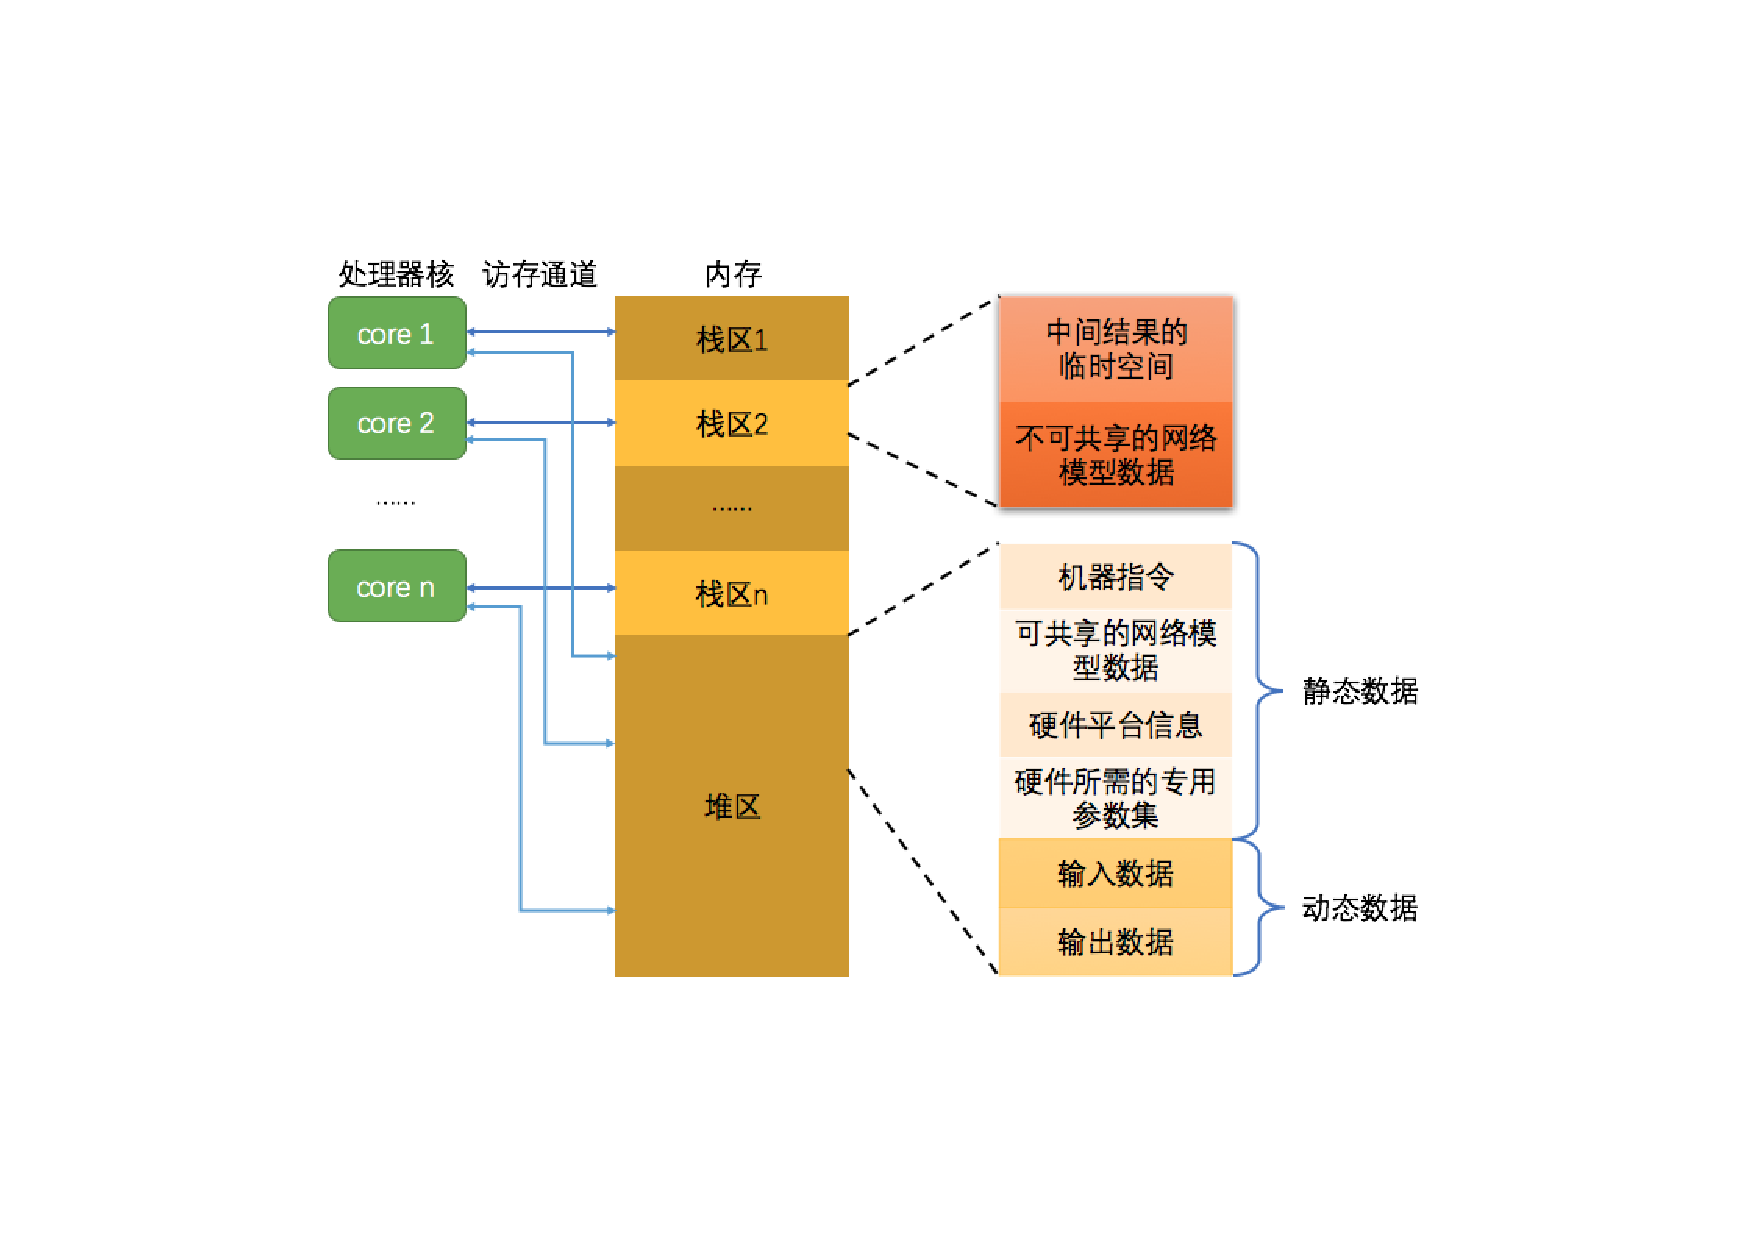
\includegraphics[width=0.6\textwidth]{general_model.pdf}
  \caption{机器学习内存布局图}
  \label{fig:general-model}
\end{figure}

生成通用深度学习模型的装置称为模型生成器(生成kernel),组成模块如图~\ref{fig:kernel-model}所示。
\begin{figure}[htb]
  \centering
  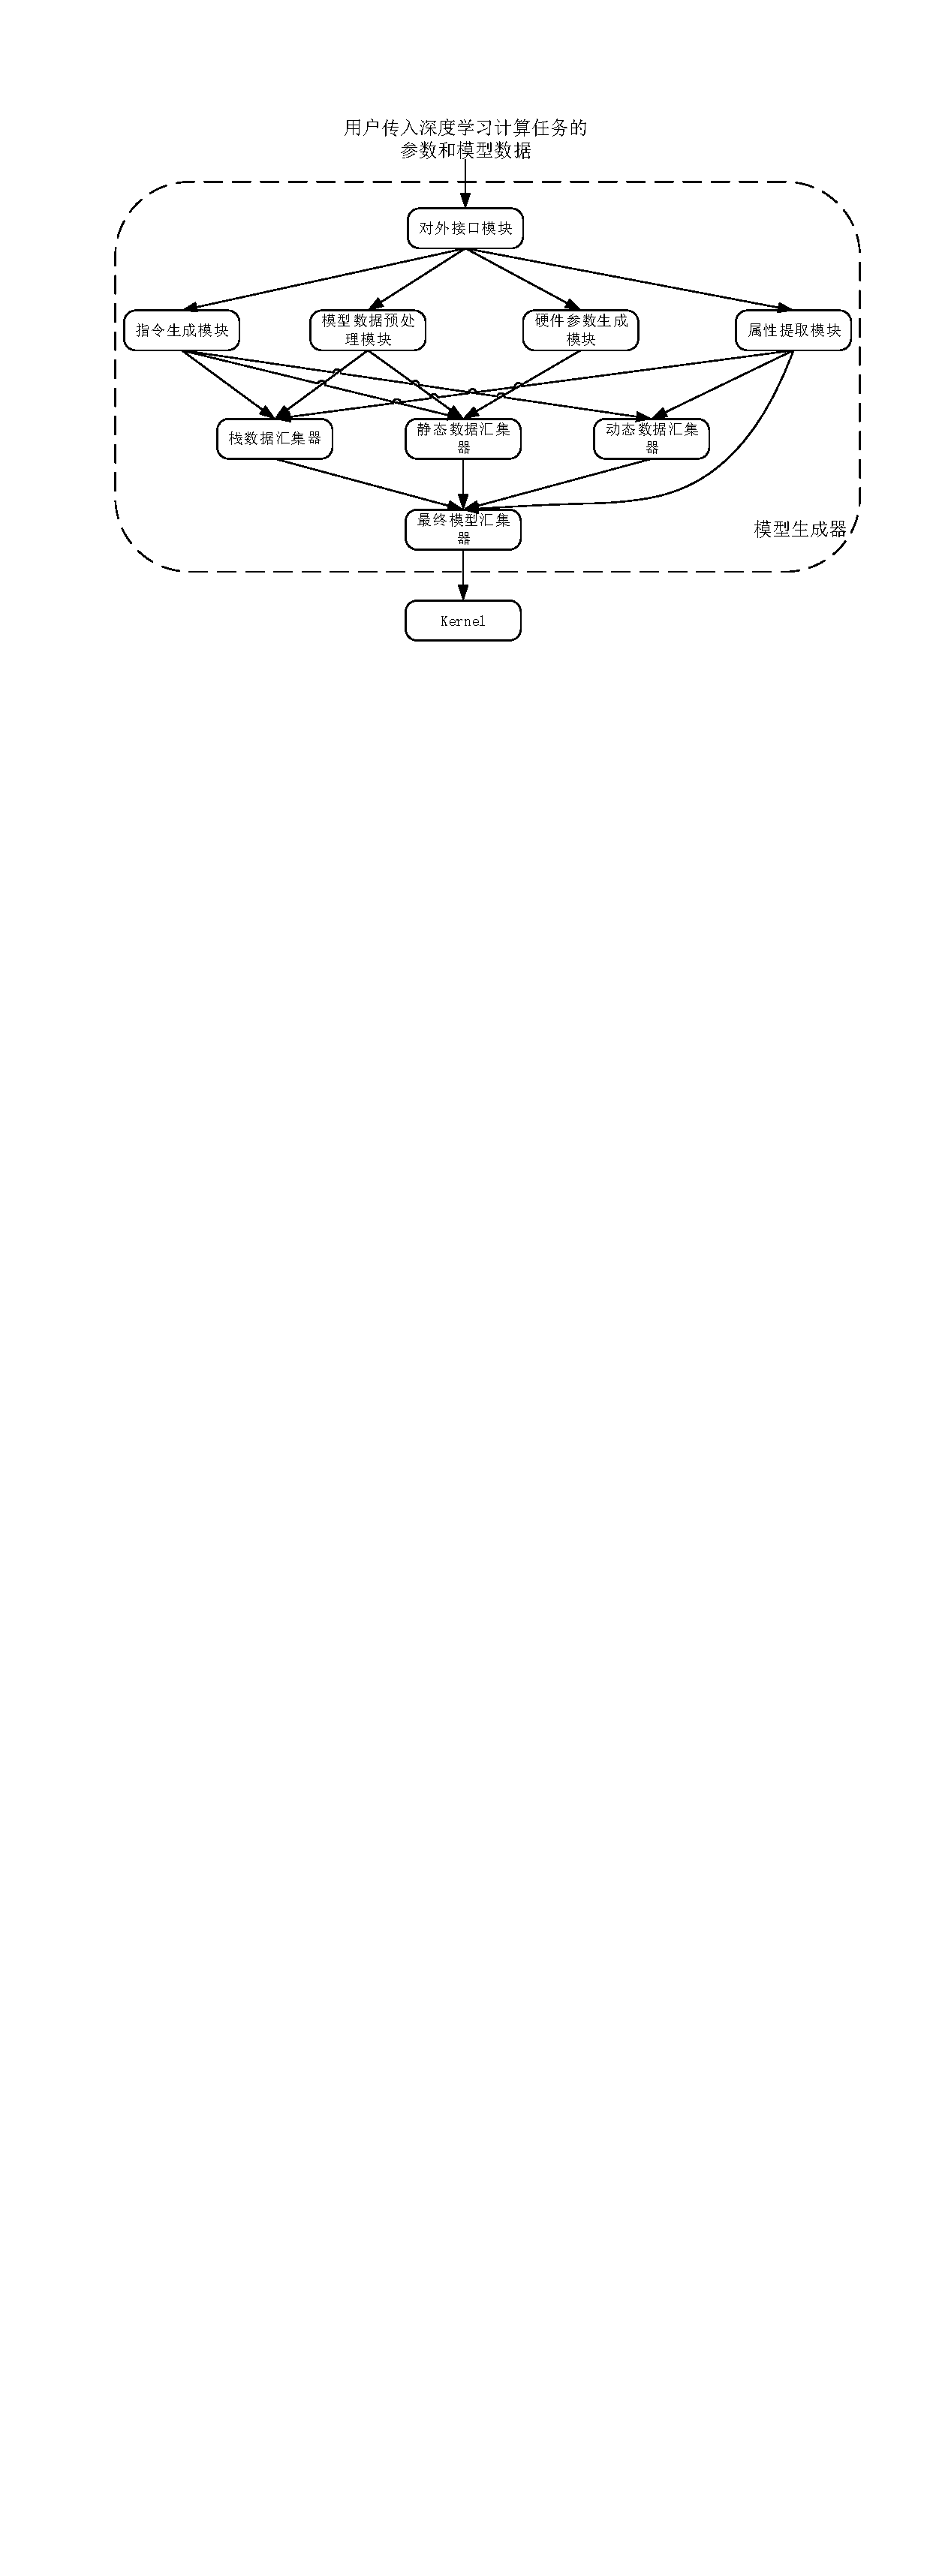
\includegraphics[width=0.8\textwidth]{kernel_model.pdf}
  \caption{kernel模块组成图}
  \label{fig:kernel-model}
\end{figure}

生成模型的步骤:
\begin{enumerate}
\item 对外接口模块接收用户传入的机器学习计算任务的参数和模型数据,将任务的参数和模型数据转换为对算法的描述信息(任务参数是用户传入的,所以不会销毁,也就是说存档),传递给指令生成模块、模型数据预处理模块、硬件参数生成模块;再将任务的参数传递给属性提取模块。
\item 指令生成模块根据算法描述信息编译生成二进制的机器指令,传递给静态数据汇集器;再计算出最佳的数据块布局传递给栈数据汇集器、静态数据汇集器、动态数据汇集器。
\item 模型数据预处理模块根据算法描述信息将机器学习模型数据做格式转换、拆分和分类,将不可共享的模型数据传递给栈数据汇集器,将共享模型数据传递给静态数据汇集器。
\item 硬件参数生成模块根据算法描述信息制造出硬件所需的专用参数集;再调用驱动程序的接口,获取硬件平台信息;然后将两者传递给静态数据汇集器。
\item 属性提取模块在机器学习计算任务的参数中提取出输入、输出数据、中间结果临时空间的属性,传递给最终模型汇集器;再从属性中提取出输入、输出数据的大小,创建各自的存储空间,传递给动态数据汇集器;再从属性中提取中间结果临时空间的大小,创建各自的存储空间,传递给栈数据汇集器。
\item 栈数据汇集器,将不可共享的模型数据和中间结果临时存储空间,根据数据块布局信息,打包整理成多段栈数据,传递给最终模型汇集器。
\item 静态数据汇集器,将机器指令、共享模型数据、硬件平台信息、硬件所需的专用参数集,根据数据块布局信息,打包整理成一段连续的静态数据,传递给最终模型汇集器。
\item 动态数据汇集器,将输入输出数据的存储空间,根据数据块布局信息,打包整理成一段连续的动态数据,传递给最终模型汇集器。
\item 最终模型汇集器,将输入输出数据和中间结果临时空间的属性、多段栈数据、连续的静态数据、连续的动态数据,合并成为一个核函数,保存在内存中。
\end{enumerate}

执行通用机器学习模型的装置模型执行器(运行核函数),其组成模块如图~\ref{fig:model-run}所示。
\begin{figure}[htb]
  \centering
  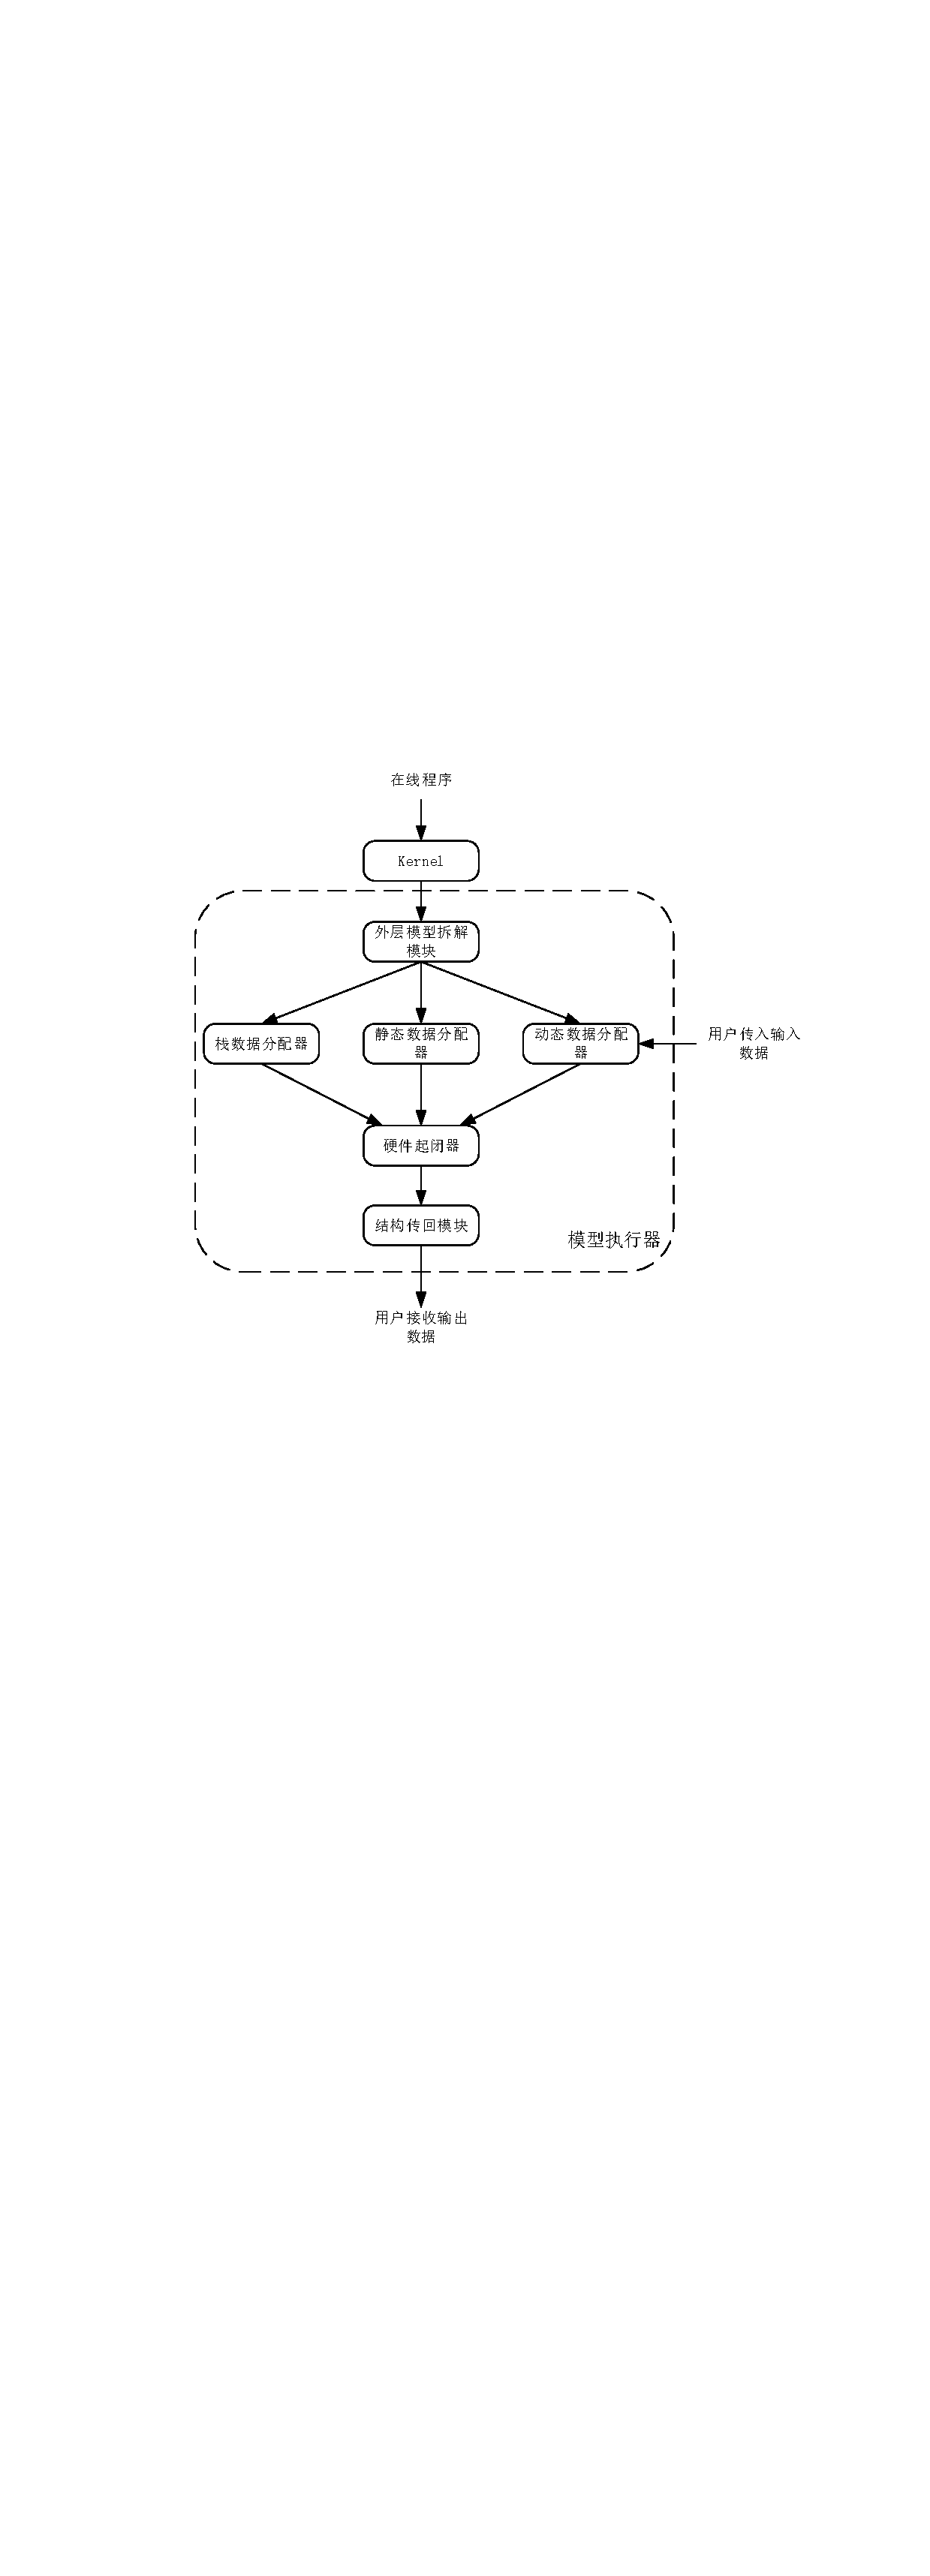
\includegraphics[width=0.6\textwidth]{model_run.pdf}
  \caption{模型执行器}
  \label{fig:model-run}
\end{figure}

执行流程:
\begin{enumerate}
\item 模型解析器读取磁盘上的离线文件,还原成内存中的核函数,传递给模型执行器。
以上步骤属于模型解析器的功能,以下步骤是模型执行器的功能。
\item 外层模型拆解模块,接收用户在线程序输入的或模型解析器给出的核函数;在其中取出输入、输出数据的属性,和一段动态数据,传递给动态数据分配器;取出中间结果临时空间的属性、多段栈数据,传递给栈数据分配器;取出静态数据,传递给静态数据分配器。
\item 栈数据分配器,在中间结果临时空间的属性中获取临时空间大小,加上每段栈数据的大小,计算出内存每个栈区需要占用的空间大小,并调用驱动程序,在各个栈区申请空间;再将每段栈数据拷入对应的栈区。
\item 静态数据分配器,根据静态数据的大小,调用驱动程序,在内存的堆区申请一块连续空间;再将静态数据拷入堆区。
\item 动态数据分配器,在输入、输出数据的属性中获取输入、输出数据大小,调用驱动程序,在内存的堆区申请多块空间(因为有可能多输入、多输出);再接收用户传入的输入数据,将它们拷入相应的堆区位置。
\item 硬件启闭器,调用驱动程序,启动硬件计算单元,开始计算;等待计算完成。
\item 结果回传模块,将输出数据从堆区取出,返回给用户。
\end{enumerate}

\subsection {指令缓存设计思路}
从上一节的介绍可以看出,kernel中保存了在设备上实现操作所需要的所有信息,想要实现指令缓存,最简单的方法就是实现kernel的离线保存和加载。所以我们可以实现一个模型保存器和一个模型解析器。模型保存器用来将多个kernel有序组织成一个离线文件,保存到磁盘中;模型解析器,用于将离线文件中的内容,还原成内存中的核函数,传递给模型执行器。

如图~\ref{fig:ins-cache-process}所示,在模型生成器生成kernel之后,利用模型保存器,将kernel保存到离线文件中。相应的,在模型执行器之前增加一个模型解析器,用于从离线文件中解析出kernel。

\begin{figure}[htb]
  \centering
  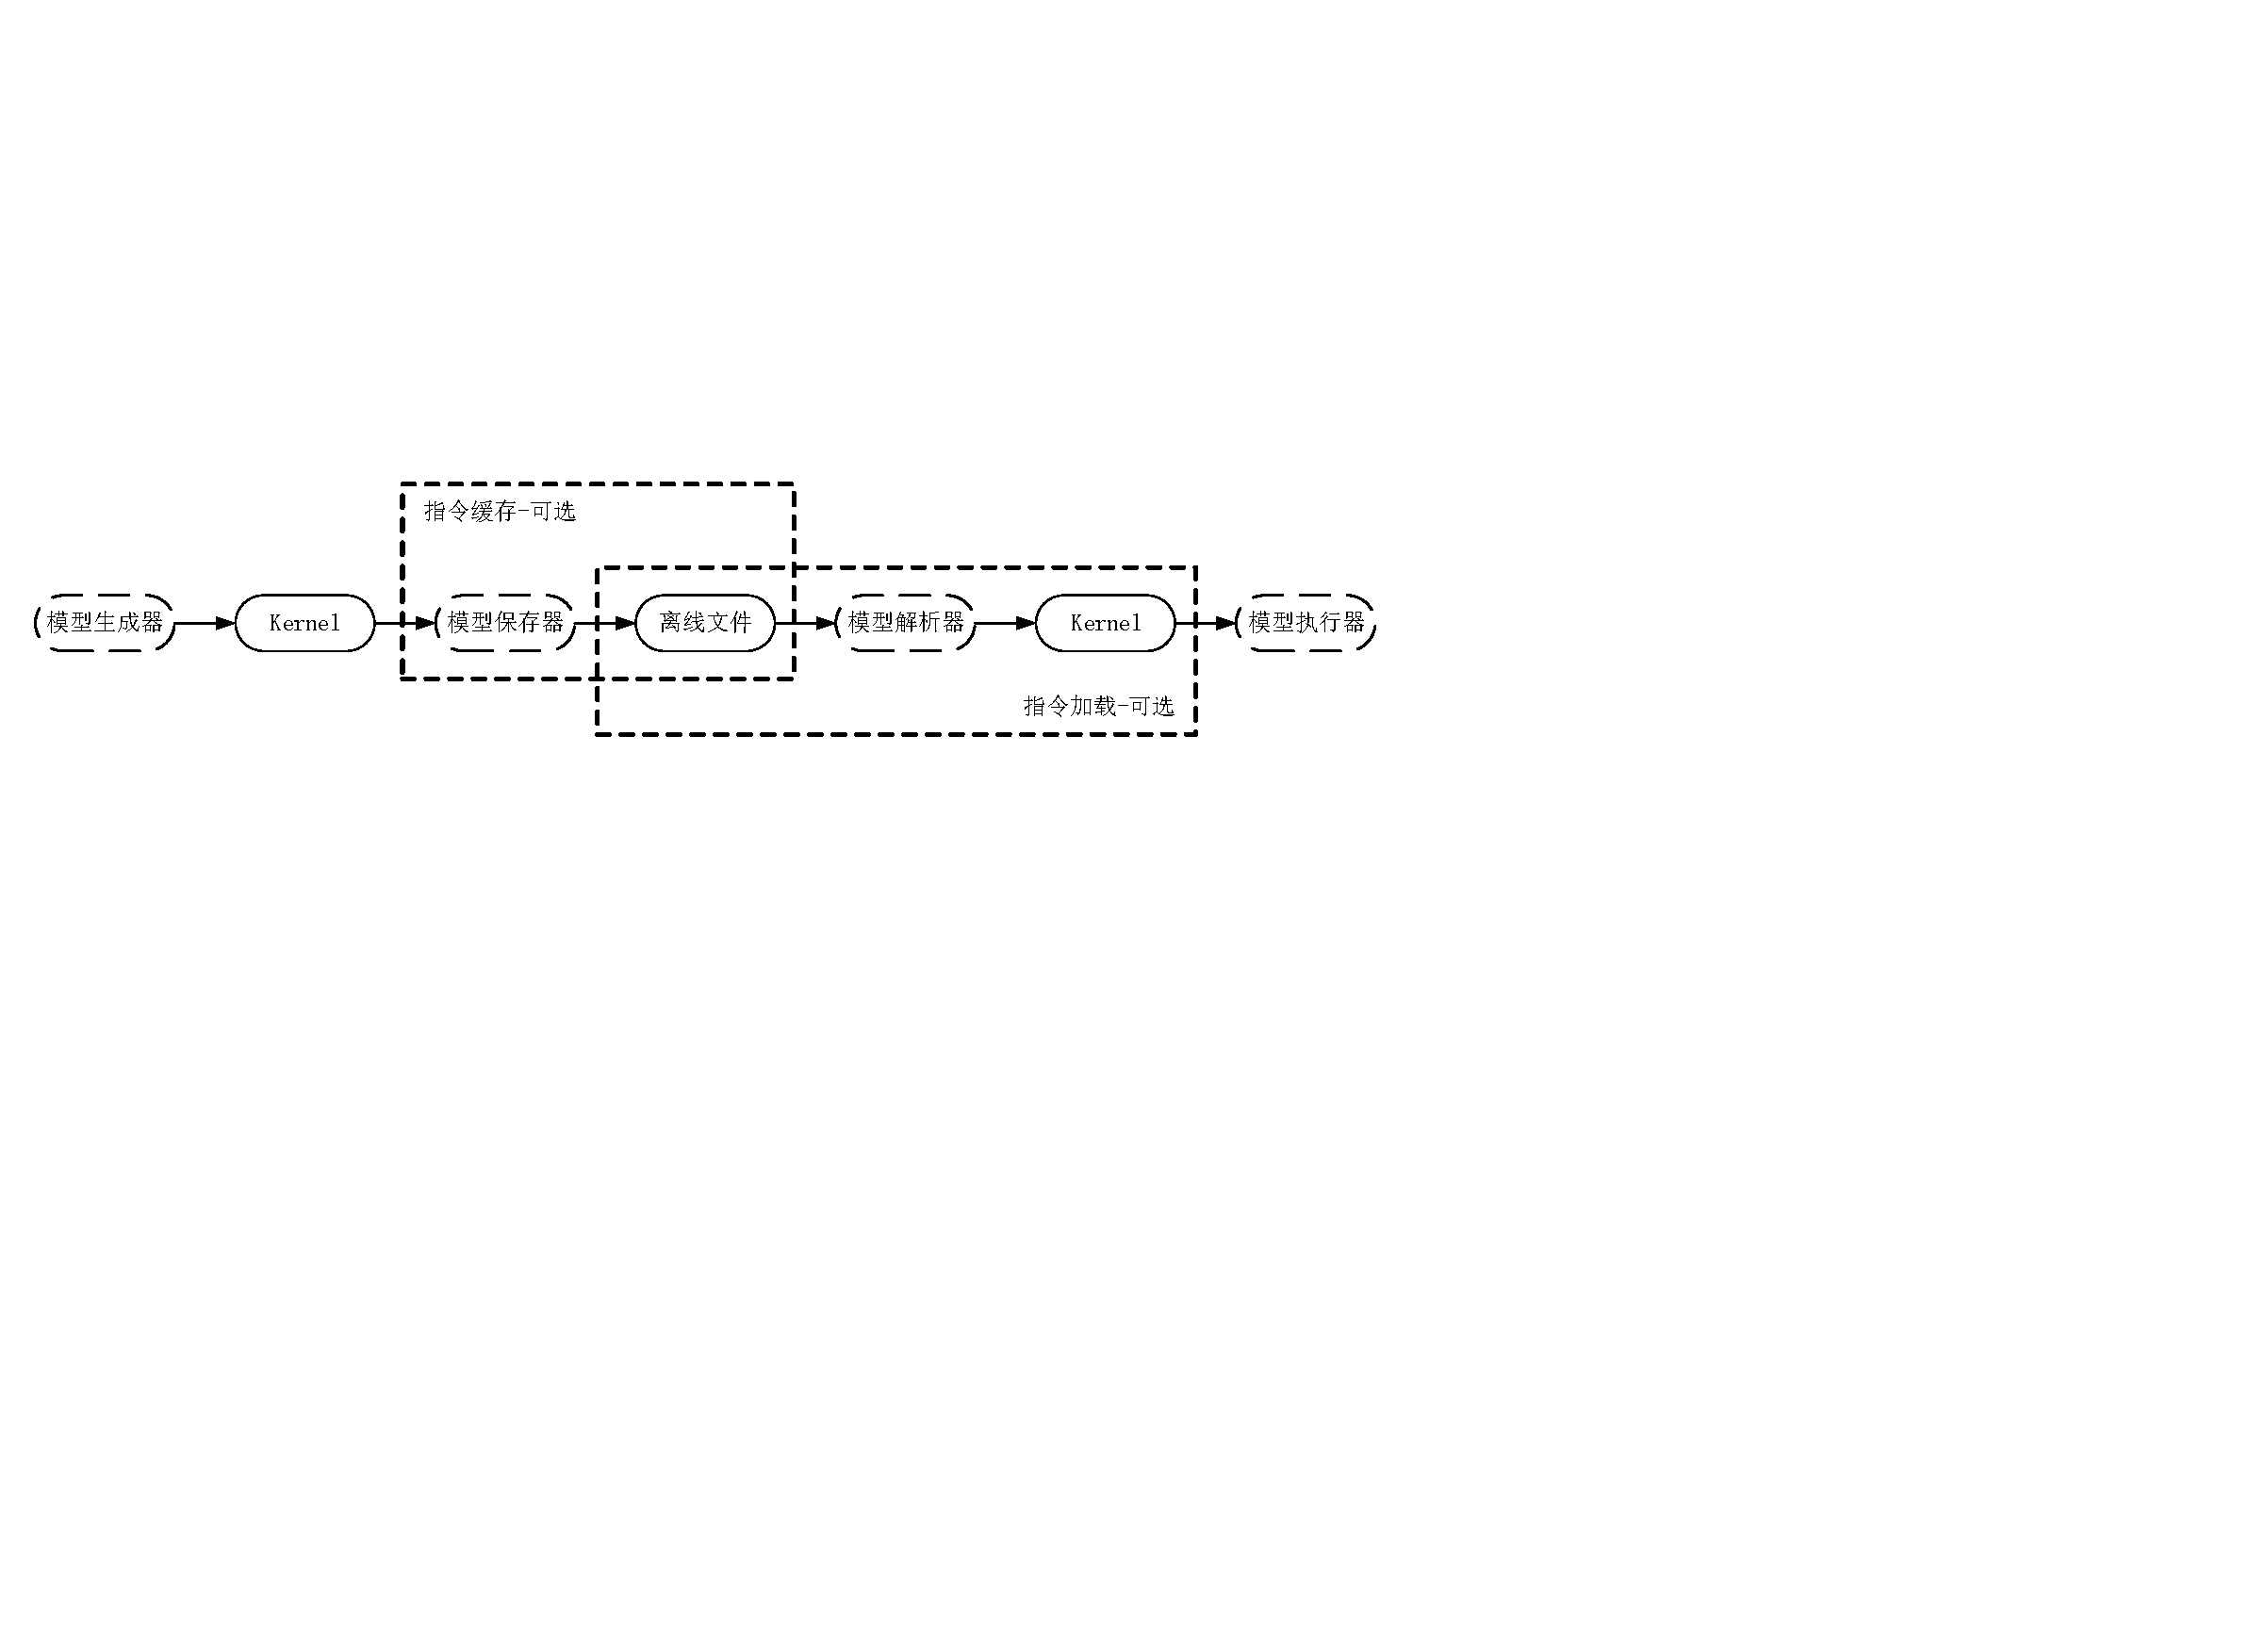
\includegraphics[width=1.0\textwidth]{ins_cache_process.pdf}
  \caption{指令缓存处理流程}
  \label{fig:ins-cache-process}
\end{figure}

所以离线模型文件是本模块的基础,离线模型文件的结构决定了模型保存器和模型生成器的处理流程,离线模型文件的结构设计如图~\ref{fig:offline-model-struct}所示。

\begin{figure}[htb]
  \centering
  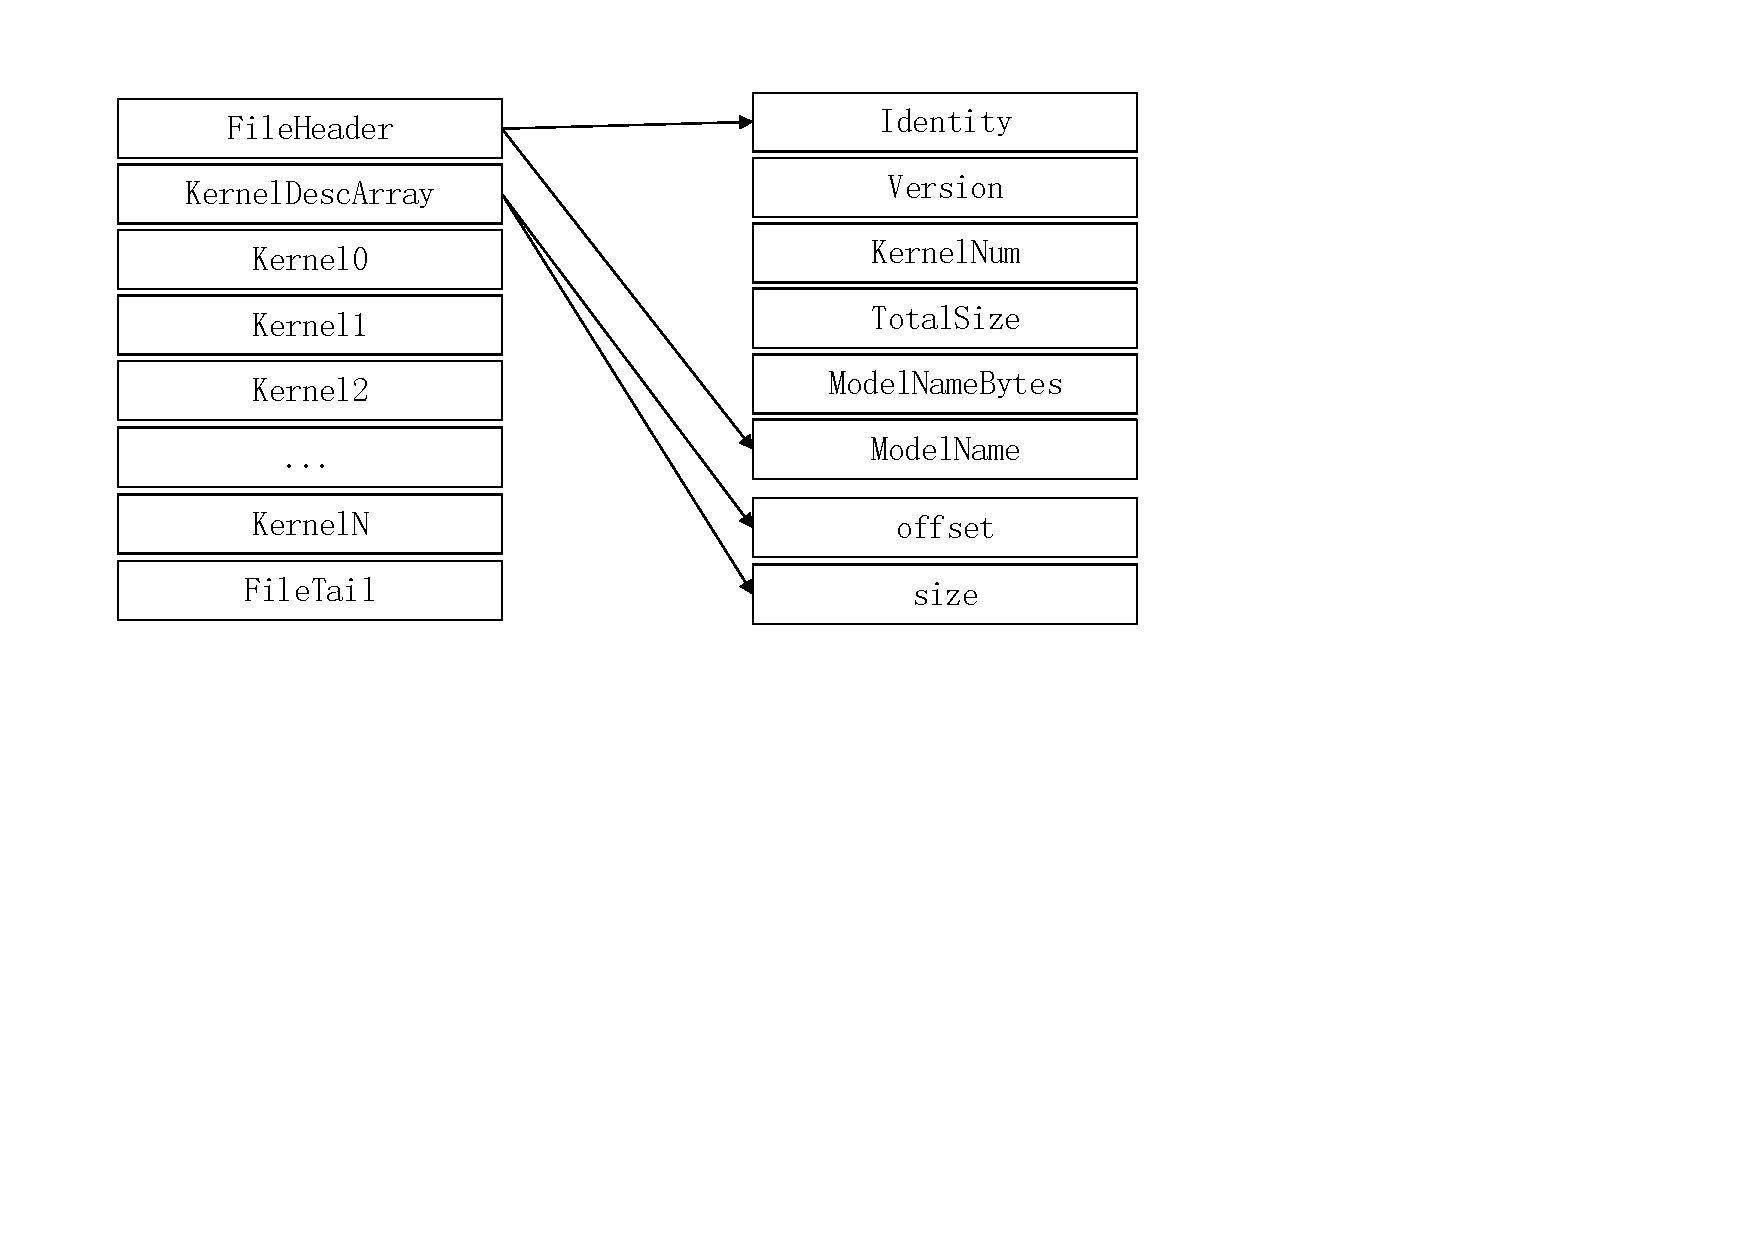
\includegraphics[width=0.6\textwidth]{offline_model_struct.pdf}
  \caption{离线模型结构}
  \label{fig:offline-model-struct}
\end{figure}

离线模型文件包含4部分:文件头,目录,具体内容,文件尾。最开始是固定大小的文件头;然后是一个数组,数据元素是kernel的描述信息,相当于文件内容的目录;紧接着是具体的kernel,保存kernel的详细信息;最后是文件尾。文件头和文件尾用于文件判别和校验,防止存储和传输图中文件的损坏;文件目录用于读取kernel的详细内容。 
文件头各部分的定义如表~\ref{tab:file-header}所示。为了解析文件的方便,FileHeader大小,为1024字节即1k,前4部分固定大小为4字节,最后用1008字节存储模型名称,空位补零填充。

\begin{table}[htb]
  \centering\small
  \caption{FileHeader结构定义}
  \label{tab:file-header}
  \begin{tabular}{llll}
    \toprule
    名称          & 类型     & 大小(字节)   & 备注       \\
    \midrule
    Identity      & string  & 4    & 文件类型检验码  \\
    Version       & string  & 4    & 离线模型版本 \\
    KernelNum     & uint64  & 4    & 文件里包含多少个kernel  \\
    TotalSize     & uint64  & 4    & 文件总大小  \\
    ModelNameBytes& uint64  & 4    & 模型名称占用多少字节  \\
    ModelName     & string  & 1008 & 模型名称  \\
    \bottomrule
  \end{tabular}
\end{table}

KernelDescArray是文件目录,实际是一个数组,数组元素是KernelDesc,数组大小和文件中保存的Kernel数量相同。KernelDesc只有两个字段:offset和size。offset当前kernel的存储位置相对于文件起始的偏移量,size表示当前kernel内容的大小。KernelDescArray可以类比于书本的目录,根据目录可以找到对应章节在哪一页,同样读文件时可以根据KernelDescArray中kernel的大小和偏移来读取指定kernel的内容。KernelDesc的定义如表~\ref{tab:kernel-desc}所示。

\begin{table}[htb]
  \centering\small
  \caption{kernelDesc定义}
  \label{tab:kernel-desc}
  \begin{tabular}{lccl}
    \toprule
    名称      & 类型     & 大小(字节)   & 备注       \\
    \midrule
    offset    & uint64  & 4    & 相对于文件头的偏移  \\
    size      & uint64  & 4    & kernel的大小 \\
    \bottomrule
  \end{tabular}
\end{table}

离线模型文件中Kernel的内容可以看作是kernel结构经过压缩和加密算法处理,序列化后生成的字符串。

FileTail中只含有一个字段,用来存储校验码,校验码的内容是根据本文件中除文件尾以外的所有内容生成的一个信息摘要编码,如表~\ref{tab:file-tail}所示。

\begin{table}[htb]
  \centering\small
  \caption{FileTail定义}
  \label{tab:file-tail}
  \begin{tabular}{lccl}
    \toprule
    名称      & 类型     & 大小(字节)   & 备注       \\
    \midrule
    CheckCode & string  & 16   & 长度为16个字符的MD5码  \\
    \bottomrule
  \end{tabular}
\end{table}

根据离线模型的定义,我们知道模型保存器应该具有模型压缩加密、计算文件大小、填充文件头、填充目录、填充kernel、填充文件尾等功能。模型保存器的组成如图~\ref{fig:mode-save}所示。

\begin{figure}[htb]
  \centering
  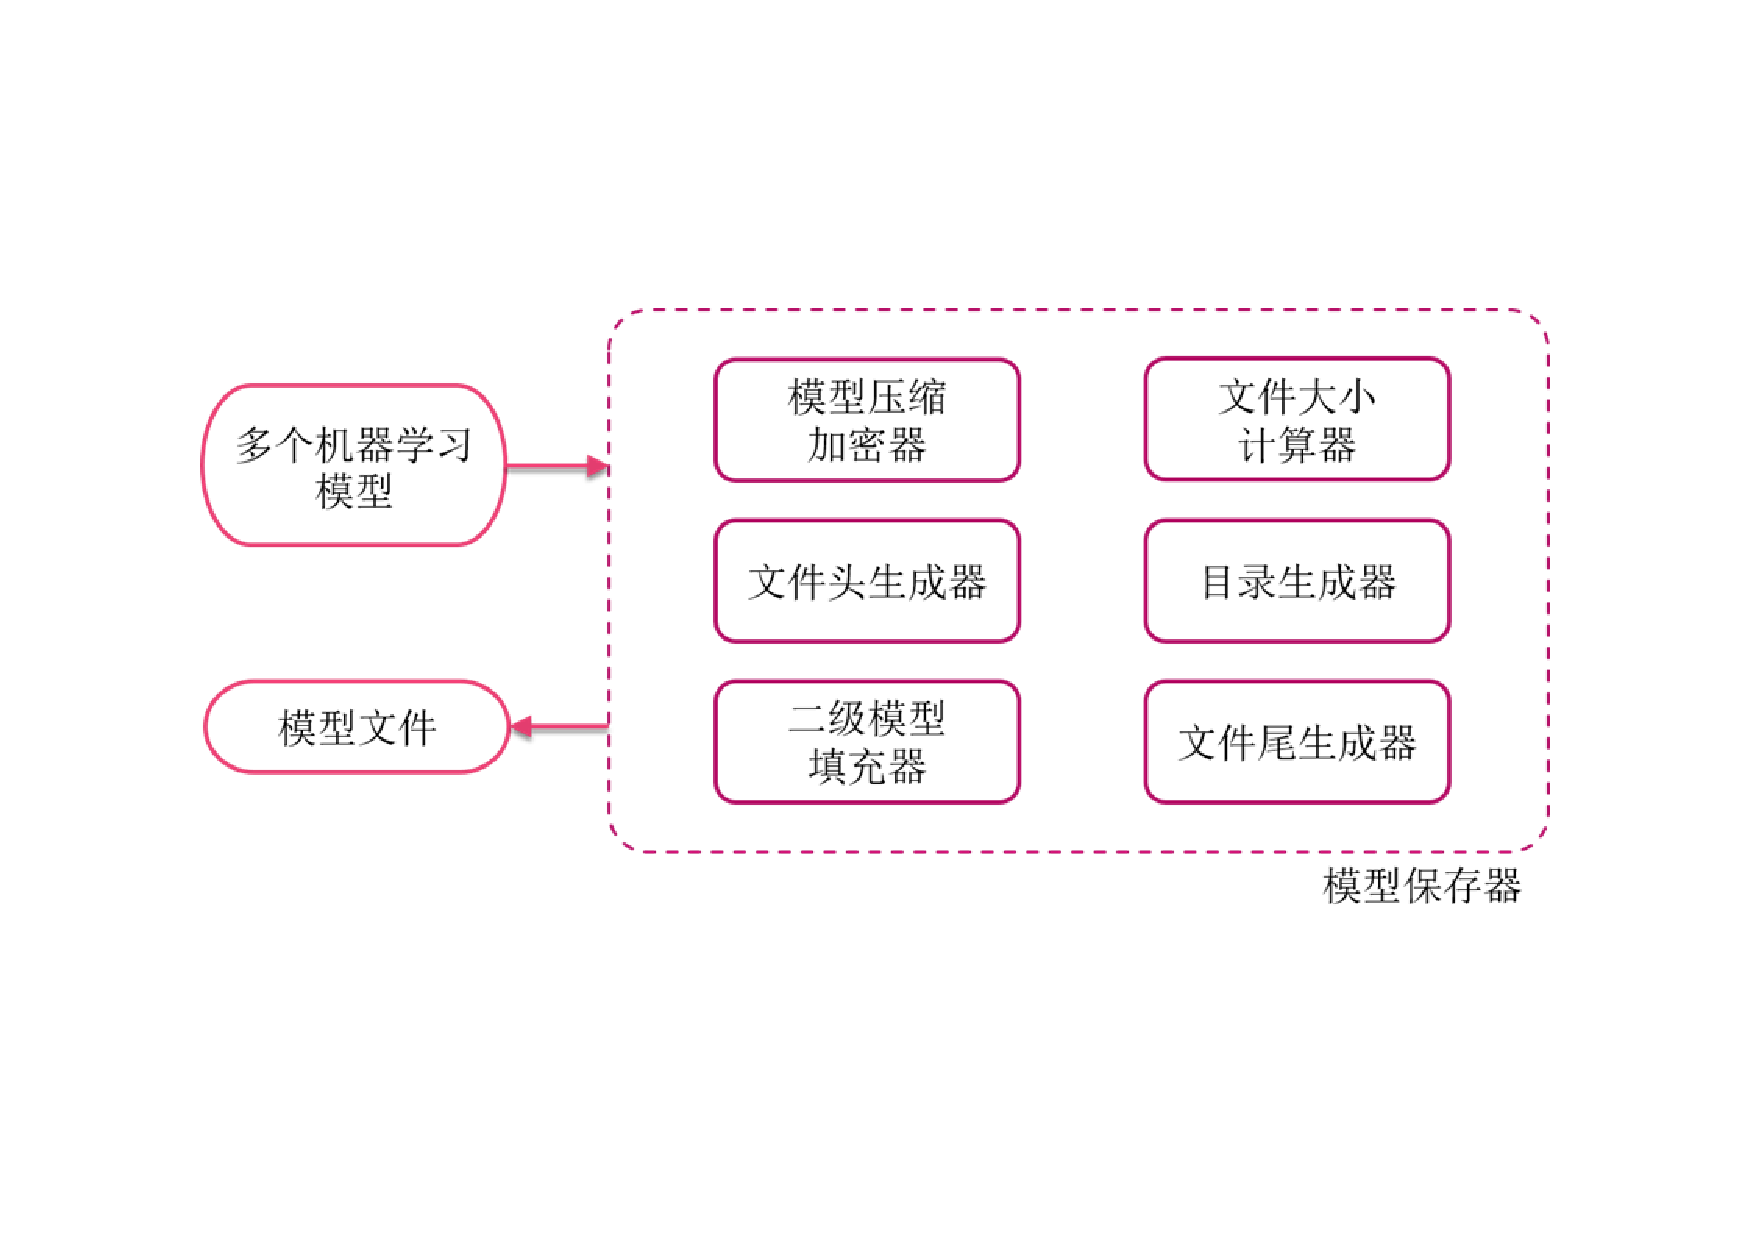
\includegraphics[width=0.8\textwidth]{model_save.pdf}
  \caption{模型保存器}
  \label{fig:mode-save}
\end{figure}

各部分的功能如下:
\begin{itemize}
  \item 模型压缩加密器用于接收多个机器学习模型,按一定压缩和加密算法对他们进行压缩和加密,得到二级模型(序列化后的字符串);
  \item 二级模型填充器用于计算每个二级模型占用存储空间的大小和模型总数量,将二级模型写入模型文件;
  \item 文件大小计算器用于接收二级模型占用存储空间的大小和模型数量,计算所有二级模型所需总大小,计算二级模型目录占用存储空间大小,加上文件头和文件尾大小,计算出模型文件总大小;
  \item 文件头生成器用于接收模型文件总大小和模型数量,产生模型文件标识码(用于区分本文件格式与其他文件不同),写入模型文件;
  \item 目录生成器用于接收二级模型占用存储空间的大小和模型数量,计算每个模型在文件中的偏移量,形成目录表,写入模型文件;
  \item 文件尾生成器将模型文件前面已写完的部分按一定算法计算校验码,写入模型文件最后,用于防止传输图中出错;
\end{itemize}

模型解析器要按照设计好的格式读取离线模型文件并解析出kernel,所以模型解析器应该具有文件校验、目录解析、模型解析等功能。模型解析器的组成如图~\ref{fig:model_praser}所示。

\begin{figure}[htb]
  \centering
  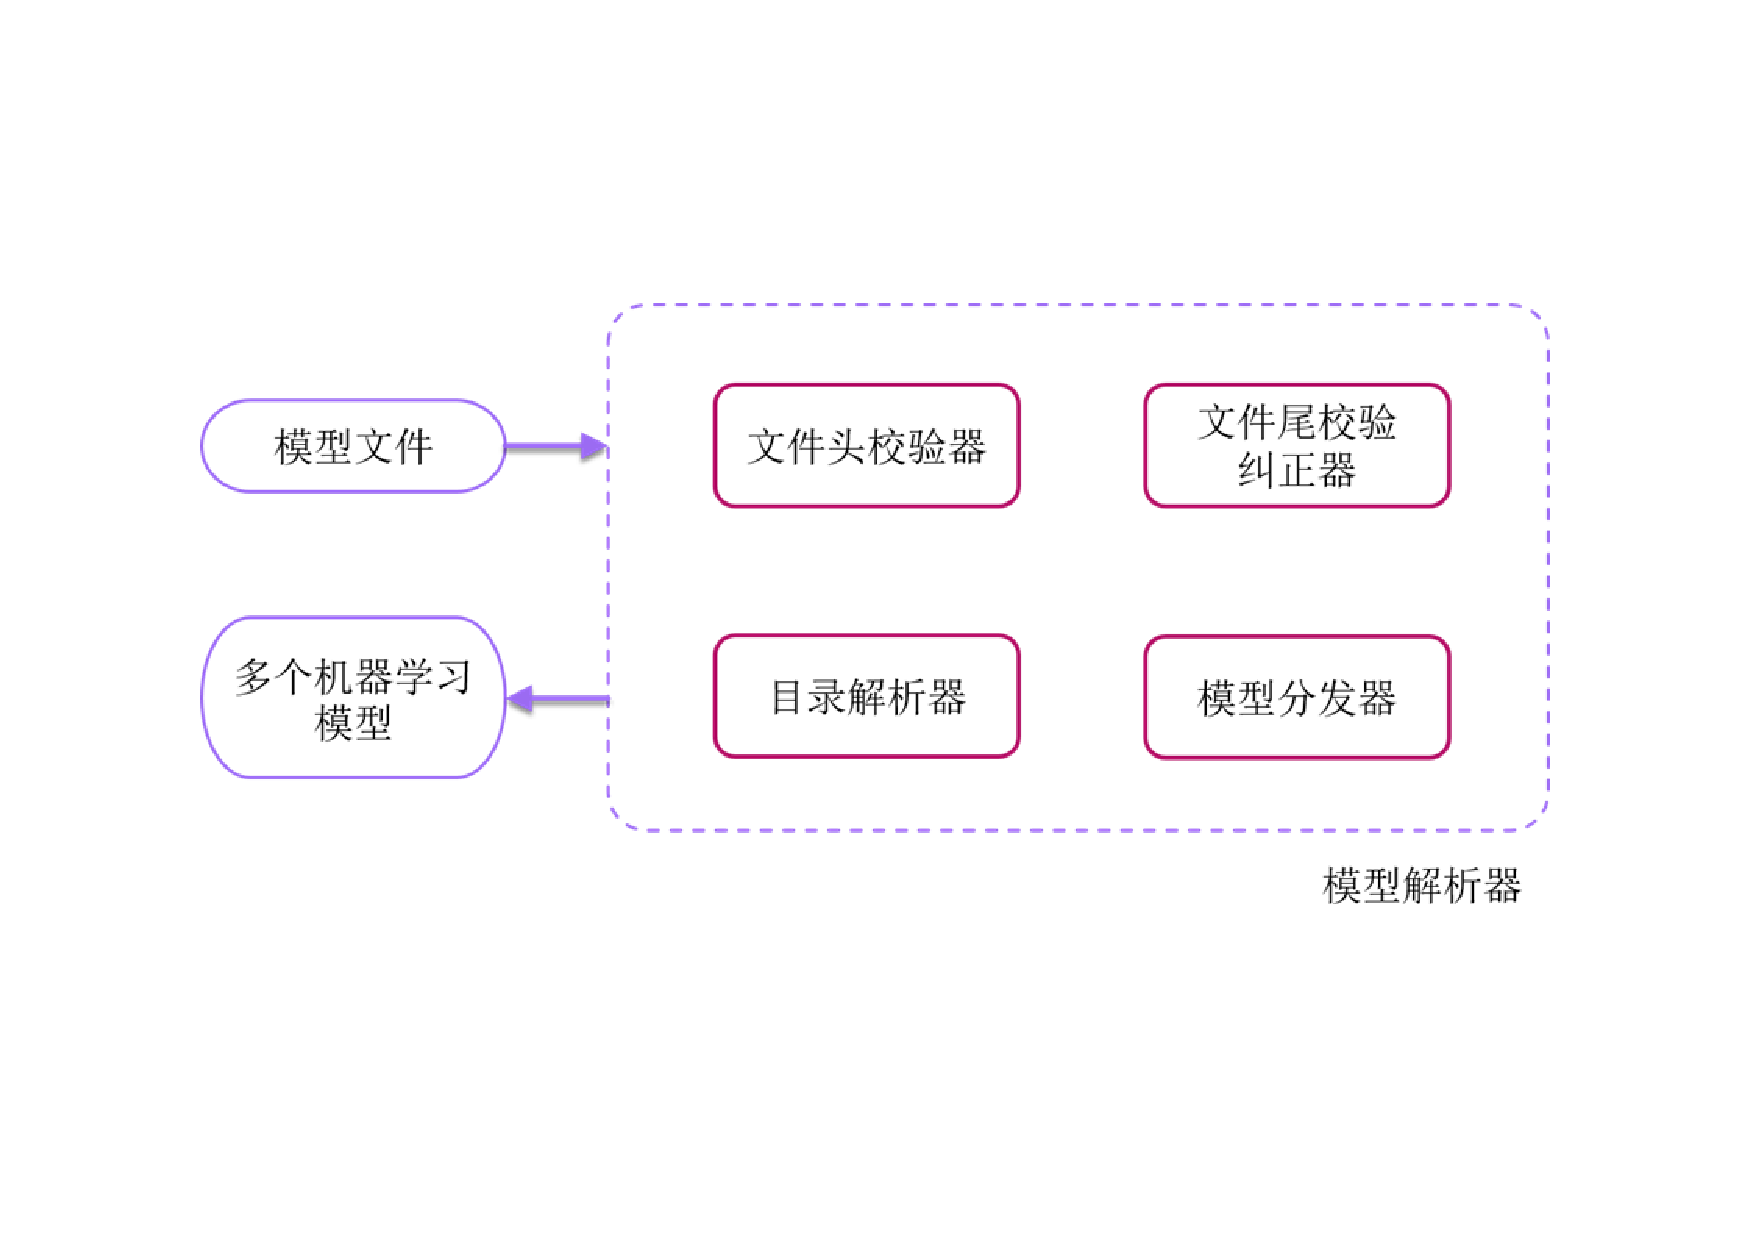
\includegraphics[width=0.8\textwidth]{model_praser.pdf}
  \caption{模型解析器}
  \label{fig:model_praser}
\end{figure}

各部分功能如下:

\begin{itemize}
  \item 文件头检验器用于读取模型文件,在文件头中找到文件标识码,检查是否合法,若合法则进入下一步,若不合法则向用户报告错误信息,解析过程停止;
  \item 文件尾校验器用于在文件尾中找到校验码,按照生成方法中相同的校验码算法,计算文件尾之前所有内容的校验码,比较本校验码与文件尾存储的校验码是否一致,若一致进行下一步,若不一致则说明文件损坏,向用户报告错误信息,解析过程停止;
  \item 目录解析器用于读取文件目录区,依次读取每个序列化后的模型,传给模型分发器;
  \item 模型分发器用于接收一个序列化后的模型,按照反序列化算法得到通用机器学习模型(kernel),然后读取通用机器学习模型中的硬件参数信息(硬件类别及型号),然后在设备池中搜索;若找到匹配硬件,则将机器学习模型发送给对应设备,由模型执行器控制后续在硬件设备上执行的过程;若找不到匹配硬件,则向用户报告错误信息,解析过程停止。(设备池可以是本机包含的计算部件,如CPU、GPU、专用处理器等,也可以是网络上可访问并可使用的计算机和计算部件)
\end{itemize}

\subsection {接口设计}

该模块对外接口的主要接口及其功能如表~\ref{tab:savemodel-interface-tab}所示。

\begin{table}[htb]
  \centering\small
  \caption{指令保存和加载模块对外接口}
  \label{tab:savemodel-interface-tab}
  \resizebox{0.6\textwidth}{36mm}{
  \begin{tabular}{ll}
    \toprule
    函数名       & saveModelToFile   \\
    \midrule
    输入 & 编译后生成的kernel \\
    输出 & 保存kernel的离线文件 \\
    功能 & 将编译后生成的指令保存到文件中\\
    说明 & 按文件设计格式填写内容 \\
    \bottomrule
    \toprule
    函数名       & loadModelFromFile    \\
    \midrule
    输入 & 离线模型的文件名 \\
    输出 & 反解析生成的kernel \\
    功能 & 从指令文件中解析出对应的kernel \\
    说明 & 解析前应做文件的完整性校验 \\
    \bottomrule
  \end{tabular}}
\end{table}

\section {权值替换模块}

\subsection {功能概述}

权值替换模块的主要目的是保持离线文件中Kernel的其它部分信息不变,只替换其权值信息的内容。该功能在网络结构信息相同,权值信息不同的时候用来替换离线模型文件中的权值数据,避免二次编译。

\subsection {设计思路}

权值信息不同肯定是Tensor绑定的数据发生了变化,由于我们并没有真正缓存权值信息对应的Json文件,而是只保存了一张权值信息表,所以我们没办法查找出具体是哪一个Tensor绑定的数据发生了变化,所以进行权值替换的时候需要将所有kernel中绑定的权值数据都进行替换。

kernel结构中包含了每个tensor的唯一标识符(name\_属性值)和绑定的静态数据信息。可以根据Tensor的名称,到kernel中找到其对应的数据,进行替换。

Tensor的name\_的属性值可以由用户通过接口显示设定,如果用户没有设定,则使用默认值,用操作名称和Tensor类型组成。如conv操作的FilterTensor默认名称是conv\_filter,conv操作的BiasTensor默认名称是conv\_bias。

\subsection {接口设计}
该模块对外接口的主要接口及其功能如表~\ref{tab:weight-replace}所示。

\begin{table}[htb]
  \centering\small
  \caption{权值替换模块对外接口}
  \label{tab:weight-replace}
  \begin{tabular}{ll}
    \toprule
    函数名       & replaceStaticData   \\
    \midrule
    输入 & 新绑定的权值数据 \\
    输出 & 更新静态数据后的kernel \\
    功能 & 更新kernel中的静态数据  \\
    说明 & 用户想要更新静态数据,必须明确指定待更新的tensor的name \\
    \bottomrule
  \end{tabular}
\end{table}

\section {权值量化模块}

\subsection {功能概述}
权值量化模块的主要功能是对浮点类型的权值数据做量化,用存储空间更小的int8或者int4类型来量化浮点数据,保证对神经网络进度影响不大的情况下,减少神经网络模型的体积,提高对缓存空间的利用率和神经网络的推理速度。

\subsection {设计思路}
现代计算机中,浮点数一般采用IEEE指定的国际标准表示,这种标准用三部分表示一个浮点数,如图~\ref{fig:float-data}所示。

\begin{figure}[htb]
  \centering
  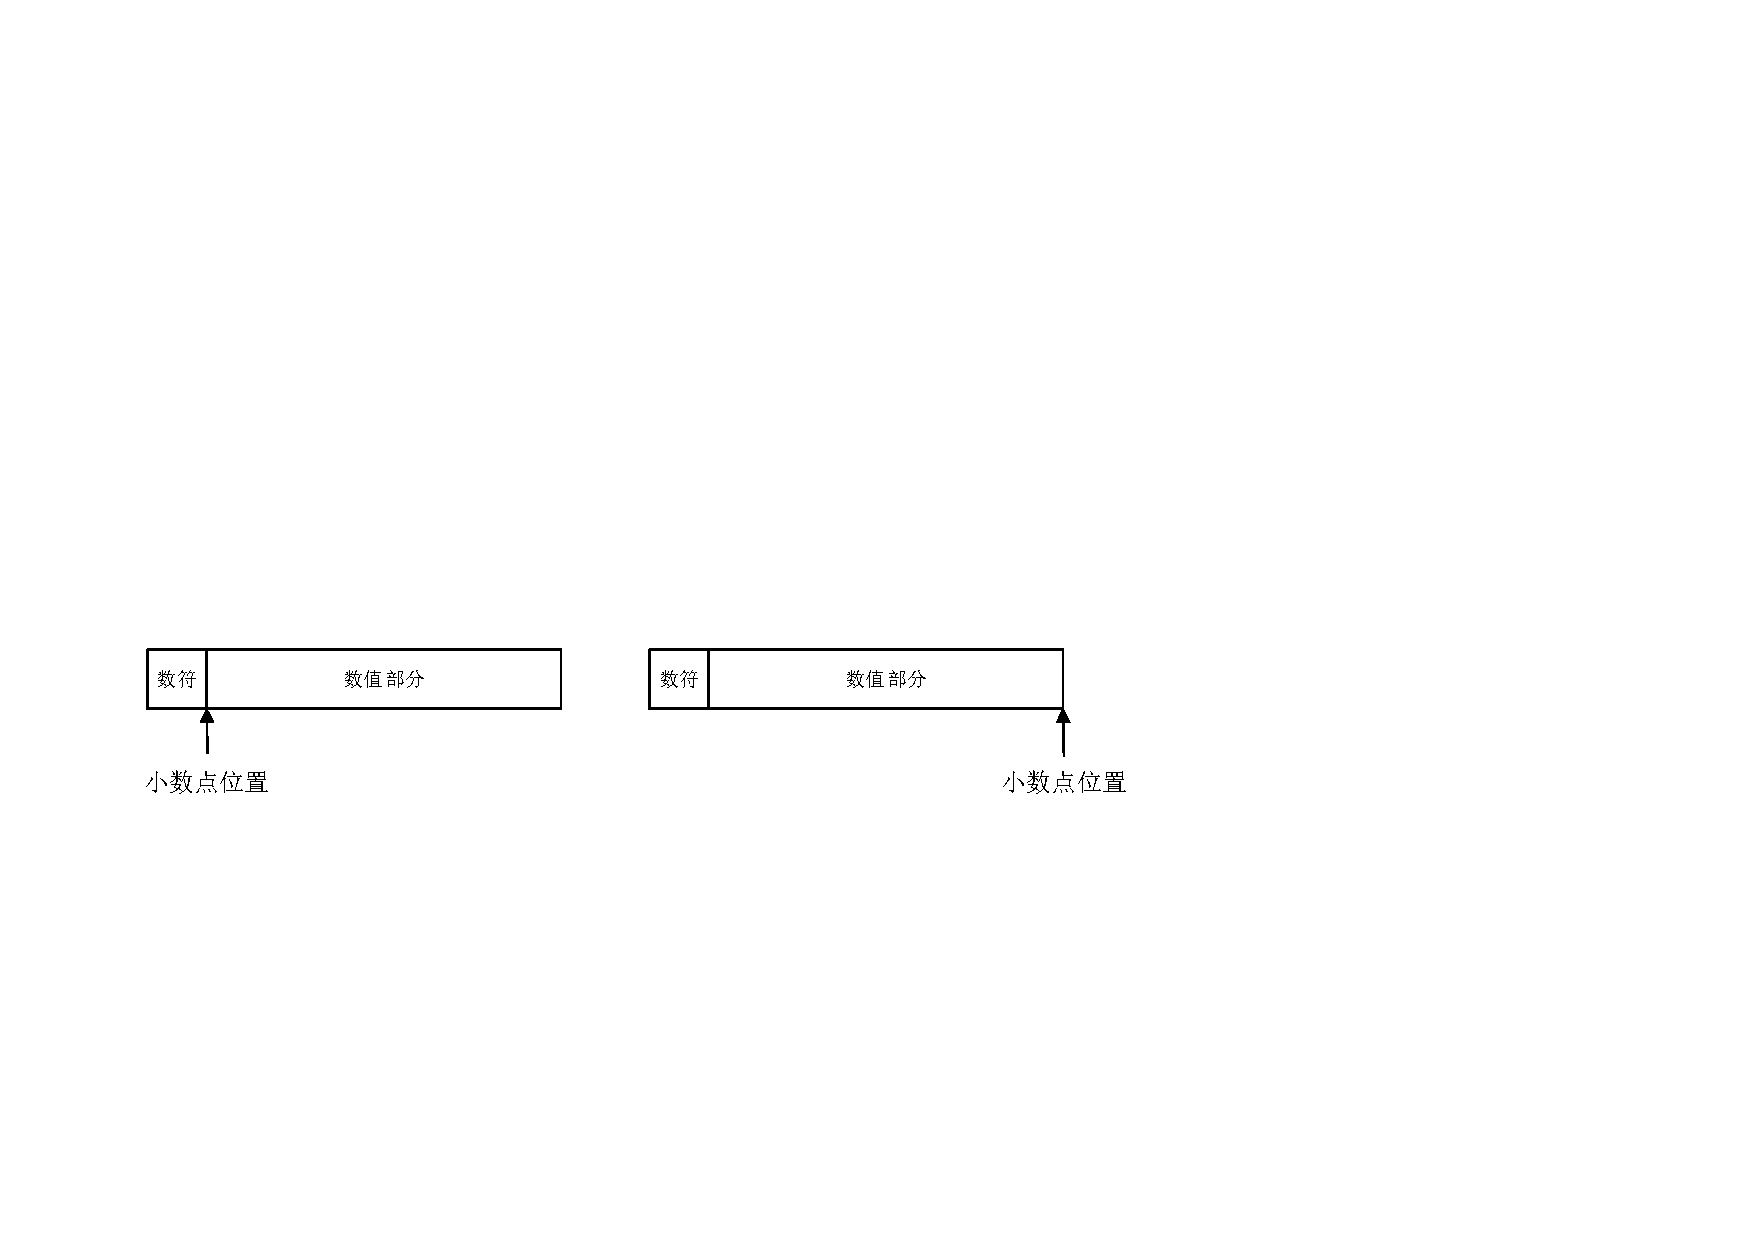
\includegraphics[width=0.8\textwidth]{float_data.pdf}
  \caption{浮点数存储示意图}
  \label{fig:float-data}
\end{figure}

数符表示浮点数的正负,用1位表示,0代表正数,1代表负数。阶码表示对浮点数进行加权,权重是2的阶码次幂,阶码的实际编码用移码表示,阶码的真实值都被加上一个常数(偏移量,float32的偏移量是127,float16的偏移量是15)后编码。尾数部分通常是规格化表示,即非0的有效位最高位总是1,但是在IEEE标准中通常会将规范化二进制浮点数整数位的1省略,称隐藏位,这样在有限的位数下,尾数可以多出一个精度位。表~\ref{tab:float32-tab}列出了十进制数178.125的实数表示。

\begin{table}[htb]
  \centering\small
  \caption{实数178.125的几种不同表示}
  \label{tab:float32-tab}
  \begin{tabular}{ll}
    \toprule
    实数表示       & 数值   \\
    \midrule
    原始十进制数   & 178.125 \\
    对应的二进制数 & 10110010.001 \\
    二进制浮点表示 & $1.0110010001^{111} $\\
    float32表示  & 符号位:0 \\ 
                 & 阶码:00000111+01111111=10000110 \\ 
                 & 尾数:01100100010000000000000(整数位1隐藏)\\
    \bottomrule
  \end{tabular}
\end{table}

小数点固定在某一位置的数称为定点数,有两种方式,如图~\ref{fig:int-data}所示。

\begin{figure}[htb]
  \centering
  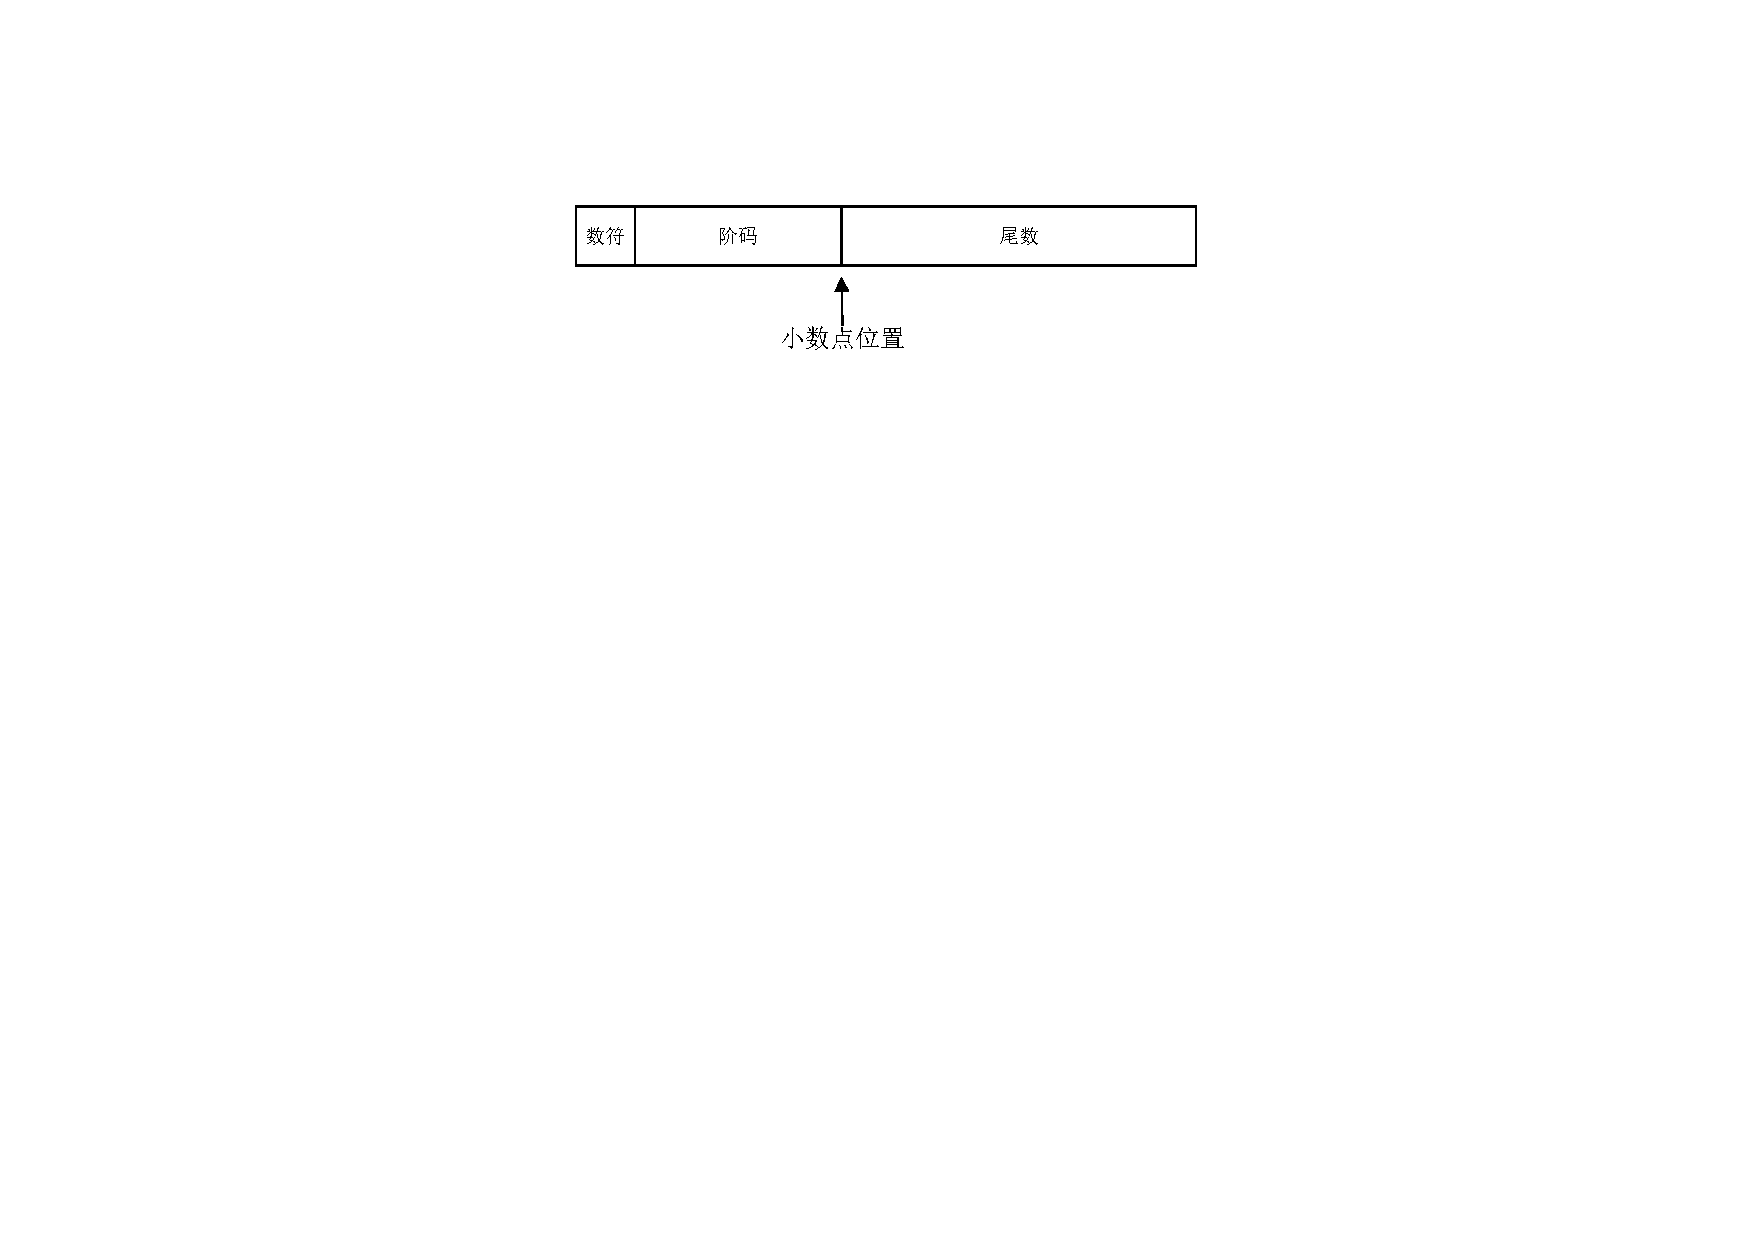
\includegraphics[width=0.6\textwidth]{int_data.pdf}
  \caption{定点数存储示意图}
  \label{fig:int-data}
\end{figure}

当小数点位于数符和第一数值位之间时为纯小数;当小数点位于数值位之后时为纯整数,数值部分的位数n决定了定点数的表示范围。如果忽略计算机内部正零和负零的表示约定,认为正零和负零是有区别的,那么纯小数的表示范围是[-(1-$2^{-n}$),1-$2^{n}$],纯整数的表示范围是[{-($2^{n}$-1}),{$2^{n}$ -1}]。

在定点数中,由于小数点的位置固定不变的,所以不能直接表示不是纯小数或者纯整数的数。但是如果我们让定点数共享一个指数,然后乘以一个比例因子,就可以表示浮点数了。

\begin{equation}
  r_x \approx q_x \times 2^{position} \times scale
\end{equation}

上述公式中,$r_x$表示真实的浮点数,$q_x$表示量化后的数值,$position$表示共享的指数,$scale$表示缩放系数。对一组浮点数进行量化的过程就是计算量化参数的过程。

\subsection {量化参数求解}

我们不妨假设对 $r_x \in \real^d$ 的实数采用n比特量化(n位纯整数),即采用n比特存储。$position$表示定点数的小数点位置,理论上在保证覆盖 $\real^d$中最大绝对值的基础上,小数点越靠左越好(小数点越靠左,精度越高),即 $position$越小越好。所以 $position$ 应该满足以下两个约束\\

\begin{equation}
  {(2^{n-1} - 1)} \times 2^{position} \ge \max r_x 
\end{equation} 

\begin{equation}
  {(2^{n-1} - 1)} \times 2^{position - 1} < \max r_x 
\end{equation} 

n比特能表示的最大的数是$2^{n-1} - 1$,量化后能表示的最大值覆盖所有需要量化的实数,又不能过大。所以\\

\begin{equation}
 log_2 {\frac {\max r_x}{2^{n-1} -1}} \le position < log_2 {\frac {\max r_x}{2^{n-1} -1}} +1
\end{equation} 
所以可以得出\\
\begin{equation}
 position = \left \lceil log_2 {\frac {\max r_x}{2^{n-1} -1}} \right \rceil  
\end{equation} 
并且可以继续推理出\\

\begin{equation}
 \frac{1}{2} < \frac {\max r_x}{{(2^{n-1} -1)} \times 2^{position}} \le 1  
\end{equation} 

其中${(2^{n-1} -1)} \times 2^{position}$表示量化能取到的最大值,然而值和实际的最大值之间有一定的差距,为了更精确的表示量化之前的数据,我们可以增加一个缩放系数$scale$来调节。所以 \\

\begin{equation}
 scale = \frac {\max r_x}{{(2^{n-1} -1)} \times 2^{position}} \Rightarrow scale \in (\frac{1}{2} \text, 1]
\end{equation} 

\subsection{接口设计}
该模块对外接口的主要接口及其功能如表~\ref{tab:weight-quant-tab}所示。

\begin{table}[htb]
  \centering\small
  \caption{权值量化模块对外接口}
  \label{tab:weight-quant-tab}
  \begin{tabular}{ll}
    \toprule
    函数名       & getPositionAndScale                \\
    \midrule
    输入 & 待量化的一组浮点数,指令量化结果类型           \\
    输出 & 量化参数position,scale的值                   \\
    功能 & 求出量化到指定类型所需要的量化参数              \\
    说明 & 量化结果类型是一个枚举变量,支持量化到不同的整型 \\
    \bottomrule
    \toprule
    函数名       & quantifyBindData              \\
    \midrule
    输入 & 用户的权值的原始数据,量化参数           \\
    输出 & 量化后的数据                            \\
    功能 & 将用户原始绑定的数据根据量化参数求进行量化 \\
    说明 & 指令文件中同时保存量化后的数据和量化参数   \\
    \bottomrule
  \end{tabular}
\end{table}

\section {本章小结}

本章主要介绍了整个框架的概要设计,根据需求分析划分出各个功能模块,然后描述了模块的主要功能,设计思路和对外接口,同时描述了系统的整体运行流程,各个模块之间的联系和依赖。通过整体的流程图和各个模块的对外接口,描述整体的实现过程和方式,为后序详细的设计奠定基础。